%% Submissions for peer-review must enable line-numbering
%% using the lineno option in the \documentclass command.
%%
%% Preprints and camera-ready submissions do not need
%% line numbers, and should have this option removed.
%%
%% Please note that the line numbering option requires
%% version 1.1 or newer of the wlpeerj.cls file, and
%% the corresponding author info requires v1.2

\documentclass[fleqn,10pt]{wlpeerj} % for preprint submissions

% ZNK -- Adding headers for pandoc

\setlength{\emergencystretch}{3em}
\providecommand{\tightlist}{
\setlength{\itemsep}{0pt}\setlength{\parskip}{0pt}}
\usepackage{lipsum}
\usepackage[unicode=true]{hyperref}
\usepackage{longtable}


% Pandoc syntax highlighting
% See https://github.com/rstudio/rticles/issues/182
\usepackage{color}
\usepackage{fancyvrb}
\newcommand{\VerbBar}{|}
\newcommand{\VERB}{\Verb[commandchars=\\\{\}]}
\DefineVerbatimEnvironment{Highlighting}{Verbatim}{commandchars=\\\{\}}
% Add ',fontsize=\small' for more characters per line
\usepackage{framed}
\definecolor{shadecolor}{RGB}{248,248,248}
\newenvironment{Shaded}{\begin{snugshade}}{\end{snugshade}}
\newcommand{\AlertTok}[1]{\textcolor[rgb]{0.94,0.16,0.16}{#1}}
\newcommand{\AnnotationTok}[1]{\textcolor[rgb]{0.56,0.35,0.01}{\textbf{\textit{#1}}}}
\newcommand{\AttributeTok}[1]{\textcolor[rgb]{0.77,0.63,0.00}{#1}}
\newcommand{\BaseNTok}[1]{\textcolor[rgb]{0.00,0.00,0.81}{#1}}
\newcommand{\BuiltInTok}[1]{#1}
\newcommand{\CharTok}[1]{\textcolor[rgb]{0.31,0.60,0.02}{#1}}
\newcommand{\CommentTok}[1]{\textcolor[rgb]{0.56,0.35,0.01}{\textit{#1}}}
\newcommand{\CommentVarTok}[1]{\textcolor[rgb]{0.56,0.35,0.01}{\textbf{\textit{#1}}}}
\newcommand{\ConstantTok}[1]{\textcolor[rgb]{0.00,0.00,0.00}{#1}}
\newcommand{\ControlFlowTok}[1]{\textcolor[rgb]{0.13,0.29,0.53}{\textbf{#1}}}
\newcommand{\DataTypeTok}[1]{\textcolor[rgb]{0.13,0.29,0.53}{#1}}
\newcommand{\DecValTok}[1]{\textcolor[rgb]{0.00,0.00,0.81}{#1}}
\newcommand{\DocumentationTok}[1]{\textcolor[rgb]{0.56,0.35,0.01}{\textbf{\textit{#1}}}}
\newcommand{\ErrorTok}[1]{\textcolor[rgb]{0.64,0.00,0.00}{\textbf{#1}}}
\newcommand{\ExtensionTok}[1]{#1}
\newcommand{\FloatTok}[1]{\textcolor[rgb]{0.00,0.00,0.81}{#1}}
\newcommand{\FunctionTok}[1]{\textcolor[rgb]{0.00,0.00,0.00}{#1}}
\newcommand{\ImportTok}[1]{#1}
\newcommand{\InformationTok}[1]{\textcolor[rgb]{0.56,0.35,0.01}{\textbf{\textit{#1}}}}
\newcommand{\KeywordTok}[1]{\textcolor[rgb]{0.13,0.29,0.53}{\textbf{#1}}}
\newcommand{\NormalTok}[1]{#1}
\newcommand{\OperatorTok}[1]{\textcolor[rgb]{0.81,0.36,0.00}{\textbf{#1}}}
\newcommand{\OtherTok}[1]{\textcolor[rgb]{0.56,0.35,0.01}{#1}}
\newcommand{\PreprocessorTok}[1]{\textcolor[rgb]{0.56,0.35,0.01}{\textit{#1}}}
\newcommand{\RegionMarkerTok}[1]{#1}
\newcommand{\SpecialCharTok}[1]{\textcolor[rgb]{0.00,0.00,0.00}{#1}}
\newcommand{\SpecialStringTok}[1]{\textcolor[rgb]{0.31,0.60,0.02}{#1}}
\newcommand{\StringTok}[1]{\textcolor[rgb]{0.31,0.60,0.02}{#1}}
\newcommand{\VariableTok}[1]{\textcolor[rgb]{0.00,0.00,0.00}{#1}}
\newcommand{\VerbatimStringTok}[1]{\textcolor[rgb]{0.31,0.60,0.02}{#1}}
\newcommand{\WarningTok}[1]{\textcolor[rgb]{0.56,0.35,0.01}{\textbf{\textit{#1}}}}

% Pandoc citation processing
\newlength{\csllabelwidth}
\setlength{\csllabelwidth}{3em}
\newlength{\cslhangindent}
\setlength{\cslhangindent}{1.5em}
% for Pandoc 2.8 to 2.10.1
\newenvironment{cslreferences}%
  {}%
  {\par}
% For Pandoc 2.11+
\newenvironment{CSLReferences}[2] % #1 hanging-ident, #2 entry spacing
 {% don't indent paragraphs
  \setlength{\parindent}{0pt}
  % turn on hanging indent if param 1 is 1
  \ifodd #1 \everypar{\setlength{\hangindent}{\cslhangindent}}\ignorespaces\fi
  % set entry spacing
  \ifnum #2 > 0
  \setlength{\parskip}{#2\baselineskip}
  \fi
 }%
 {}
\usepackage{calc} % for calculating minipage widths
\newcommand{\CSLBlock}[1]{#1\hfill\break}
\newcommand{\CSLLeftMargin}[1]{\parbox[t]{\csllabelwidth}{#1}}
\newcommand{\CSLRightInline}[1]{\parbox[t]{\linewidth - \csllabelwidth}{#1}\break}
\newcommand{\CSLIndent}[1]{\hspace{\cslhangindent}#1}

% Pandoc Header
\usepackage{lipsum} \usepackage[htt]{hyphenat} \usepackage{booktabs} \usepackage{microtype}

\usepackage{flafter}
\usepackage{booktabs}
\usepackage{longtable}
\usepackage{array}
\usepackage{multirow}
\usepackage{wrapfig}
\usepackage{float}
\usepackage{colortbl}
\usepackage{pdflscape}
\usepackage{tabu}
\usepackage{threeparttable}
\usepackage{threeparttablex}
\usepackage[normalem]{ulem}
\usepackage{makecell}
\usepackage{xcolor}

\title{shorts: An R Package for Modeling Short Sprints}

\author[1]{Mladen Jovanović}

\corrauthor[1]{Mladen Jovanović}{\href{mailto:coach.mladen.jovanovic@gmail.com}{\nolinkurl{coach.mladen.jovanovic@gmail.com}}}
\author[2]{Jason D. Vescovi}


\affil[1]{Faculty of Sport and Physical Education, University of Belgrade, Serbia}
\affil[2]{Faculty of Kinesiology and Physical Education, Graduate School of Exercise Science, Toronto, ON Canada}


%
% \author[1]{First Author}
% \author[2]{Second Author}
% \affil[1]{Address of first author}
% \affil[2]{Address of second author}
% \corrauthor[1]{First Author}{f.author@email.com}

% 

\begin{abstract}
Short sprint performance is one of the most distinguishable and admired physical traits in sports. Short sprints have been modeled using the mono-exponential equation that involves two parameters: (1) maximum sprinting speed (MSS) and (2) relative acceleration (TAU). The most common methods to assess short sprint performance are with a radar gun or timing gates. In this paper, we: 1) provide the \textbf{shorts} package that can model sprint timing data from these two sources; 2) discuss potential issues with assessing sprint time (synchronization and flying start, respectively); and 3) provide model definitions within the \textbf{shorts} package to help alleviate errors within the subsequent parameter outcomes.
% Dummy abstract text. Dummy abstract text. Dummy abstract text. Dummy abstract text. Dummy abstract text. Dummy abstract text. Dummy abstract text. Dummy abstract text. Dummy abstract text. Dummy abstract text. Dummy abstract text.
\end{abstract}

\begin{document}

\flushbottom
\maketitle
\thispagestyle{empty}

\hypertarget{introduction}{%
\section{Introduction}\label{introduction}}

Short sprint performance is one of the most distinguishable and admired physical traits in sports. Short sprints, commonly performed in most team sports (e.g., soccer, field hockey, handball, football, etc.), are defined as maximal running from a stand still position over a distance that doesn't result in deceleration at the end. Peak anaerobic power is achieved within the first few seconds (\textless5 s) of maximal efforts (\protect\hyperlink{ref-mangineSpeedForcePower2014}{Mangine et al. 2014}), whereas the ability to achieve maximal sprint speed varies based on the type of sport. For example, track and field sprinters are trained to achieve maximal speed later in a race (i.e., 50-60 m) (\protect\hyperlink{ref-ward-smithEnergyConversionStrategies2001}{Ward-Smith 2001}), but team sport athletes have sport-specific attributes and reach it much sooner (i.e., 30-40 m)(\protect\hyperlink{ref-brownAssessmentLinearSprinting2004}{Brown, Vescovi, and Vanheest 2004}). Regardless of the differences in kinematics between athletes, evaluating short sprint performance is routinely included within a battery of fitness tests for a wide range of sports

The use of force plates is considered the gold standard for assessing mechanical properties of sprinting; however, there are logistical and financial challenges to capturing the profile of an entire sprint (\protect\hyperlink{ref-morinSimpleMethodComputing2019}{Jean-Benoit Morin et al. 2019}; \protect\hyperlink{ref-samozinoSimpleMethodMeasuring2016}{Samozino et al. 2016}). Radar and laser technology are frequently used laboratory-grade methods (\protect\hyperlink{ref-buchheitMechanicalDeterminantsAcceleration2014}{Buchheit et al. 2014}; \protect\hyperlink{ref-edwardsSprintAccelerationCharacteristics2020}{Edwards et al. 2020}; \protect\hyperlink{ref-jimenez-reyesRelationshipVerticalHorizontal2018}{Jiménez-Reyes et al. 2018}; \protect\hyperlink{ref-marcote-pequenoAssociationForceVelocity2019}{Marcote-Pequeño et al. 2019}) but not normally accessible to practitioners working in sports. Undoubtedly, the most common method available and used to evaluate sprint performance are timing gates. Often multiple gates are positioned at varying distances to capture split times (e.g., 5, 10, 20 m), which can now be incorporated into the method for determining sprint mechanical properties (\protect\hyperlink{ref-morinSimpleMethodComputing2019}{Jean-Benoit Morin et al. 2019}; \protect\hyperlink{ref-samozinoSimpleMethodMeasuring2016}{Samozino et al. 2016}). This approach presents an advantage to practitioners who can use the outcomes to describe individual differences, quantify the effects of training interventions, and better understanding the limiting factors of performance.

The \textbf{shorts} package (\protect\hyperlink{ref-R-shorts}{Jovanović 2021}), written in the R language (\protect\hyperlink{ref-R-base}{R Core Team 2020}), represents an open-source tool to help sports scientists translate raw timing data into detailed mechanical outcomes through mathematical modeling (\protect\hyperlink{ref-morinSimpleMethodComputing2019}{Jean-Benoit Morin et al. 2019}; \protect\hyperlink{ref-samozinoSimpleMethodMeasuring2016}{Samozino et al. 2016}). To best of our knowledge, scientist, researchers, and coaches have been performing short sprints modeling using the built-in solver function of Excel (Microsoft Corporation, Redmond, Washington, United States) (\protect\hyperlink{ref-morinSpreadsheetSprintAcceleration2017}{J. B. Morin 2017}; \protect\hyperlink{ref-morinSpreadsheetSprintAcceleration2019}{Jean-Benoit Morin and Samozino 2019}; \protect\hyperlink{ref-stenrothForcevelocityProfilingIce2020}{Stenroth, Vartiainen, and Karjalainen 2020}; \protect\hyperlink{ref-stenrothSpreadsheetSprintAcceleration2020}{Stenroth and Vartiainen 2020}; \protect\hyperlink{ref-samozinoSimpleMethodMeasuring2016}{Samozino et al. 2016}; \protect\hyperlink{ref-clarkNFLCombine40Yard2017}{Clark et al. 2017}; \protect\hyperlink{ref-morinSimpleMethodComputing2019}{Jean-Benoit Morin et al. 2019}), which makes the \textbf{shorts} package a major improvement in ease-of-use, speed, transparency, reproducibility, and more feature-rich model fitting.

In the current paper, we will provide an explanation of one commonly used mathematical equation to model short sprints, modeling applications using the \textbf{shorts} package, issues that can arise during measurement and estimation, and potential solutions to those problems.

\hypertarget{mathematical-model}{%
\section{Mathematical model}\label{mathematical-model}}

Short sprints have been modeled using the mono-exponential equation \eqref{eq:velocity-time} originally proposed by \protect\hyperlink{ref-doi:10.1098ux2frspb.1927.0035}{Furusawa, Hill, and Parkinson} (\protect\hyperlink{ref-doi:10.1098ux2frspb.1927.0035}{1927}), and more recently popularized by \protect\hyperlink{ref-clarkNFLCombine40Yard2017}{Clark et al.} (\protect\hyperlink{ref-clarkNFLCombine40Yard2017}{2017}), and \protect\hyperlink{ref-samozinoSimpleMethodMeasuring2016}{Samozino et al.} (\protect\hyperlink{ref-samozinoSimpleMethodMeasuring2016}{2016}). Equation \eqref{eq:velocity-time} represents function for instantaneous horizontal velocity \(v\) given the time \(t\) and two model parameters:

\begin{equation}
  v(t) = MSS \times (1 - e^{-\frac{t}{TAU}}) \label{eq:velocity-time}
\end{equation}

The parameters of the equation \eqref{eq:velocity-time} are \emph{maximum sprinting speed} (MSS; expressed in \(ms^{-1}\)) and \emph{relative acceleration} (TAU). Mathematically, TAU represents the ratio of MSS to initial acceleration (MAC; \emph{maximal acceleration}, expressed in \(ms^{-2}\)) \eqref{eq:maximal-acceleration}.

\begin{equation}
  MAC = \frac{MSS}{TAU}\label{eq:maximal-acceleration}
\end{equation}

Although TAU is used in the equations, and later estimated, we prefer to use MAC instead since it is easier to grasp, particularly for less math inclined coaches.

By derivating equation \eqref{eq:velocity-time}, we can get equation for horizontal acceleration \eqref{eq:acceleration-time}.

\begin{equation}
  a(t) = \frac{MSS}{TAU} \times e^{-\frac{t}{TAU}}  \label{eq:acceleration-time}
\end{equation}

By integrating equation \eqref{eq:velocity-time}, we can get equation for distance covered \eqref{eq:distance-time}.

\begin{equation}
  d(t) = MSS \times (t + TAU \times e^{-\frac{t}{TAU}}) - MSS \times TAU  \label{eq:distance-time}
\end{equation}

Let's consider four athletes with different levels of MSS (high versus low maximal sprinting speed) and MAC (high versus low maximal acceleration; as mentioned previously, using MAC is preferred over using TAU) (Table \ref{tab:four-athletes-table}).

\small

\begin{table}

\caption{\label{tab:four-athletes-table}Four athletes with different MSS and MAC parameters.}
\centering
\begin{tabular}[t]{lrrr}
\toprule
Athlete & MSS & MAC & TAU\\
\midrule
Athlete A & 12 & 10 & 1.20\\
Athlete B & 12 & 6 & 2.00\\
Athlete C & 8 & 10 & 0.80\\
Athlete D & 8 & 6 & 1.33\\
\bottomrule
\end{tabular}
\end{table}

\normalsize

Figure \ref{fig:four-athletes-kinematics} depicts distance, velocity, and acceleration over time (from 0 to 6 s).

\small

\begin{figure}

{\centering 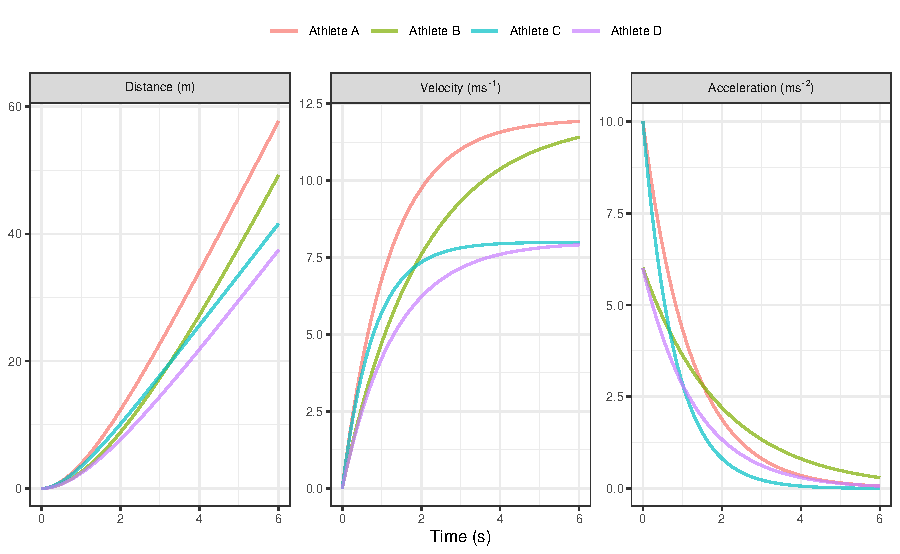
\includegraphics[width=0.9\linewidth]{paper_files/figure-latex/four-athletes-kinematics-1} 

}

\caption{Kinematic characteristic of four athletes with different MSS and MAC parameters over a period of 0 to 6 seconds.}\label{fig:four-athletes-kinematics}
\end{figure}

\normalsize

Plotting acceleration against velocity (Figure \ref{fig:four-athletes-profile}), we will get \emph{Acceleration-Velocity Profile}, which is linear, according to the mathematical model. If the athlete's body mass (kg) is known, as well as additional air resistance parameters (see \protect\hyperlink{air-resistance-and-the-calculation-of-force-and-mechanical-power}{Air resistance and the calculation of force and mechanical power} section of this paper), \emph{Force-Velocity Profile} can be estimated (see \protect\hyperlink{force-velocity-profile}{Force-Velocity profile} section of this paper).

\small

\begin{figure}

{\centering 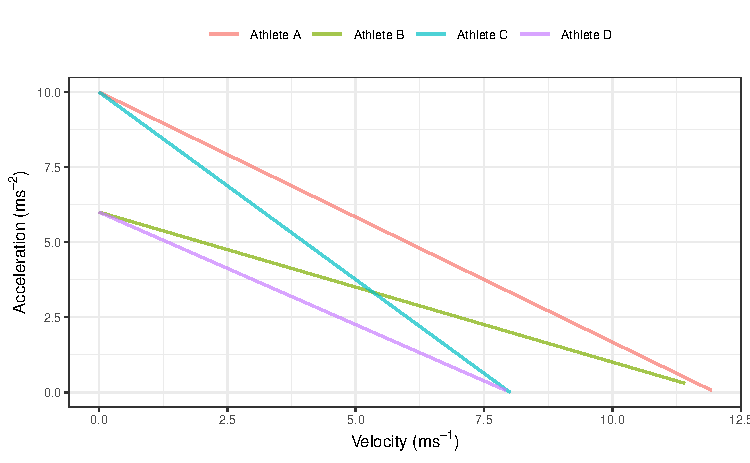
\includegraphics[width=0.9\linewidth]{paper_files/figure-latex/four-athletes-profile-1} 

}

\caption{Acceleration-Velocity profile of four athletes with different MSS and MAC parameters.}\label{fig:four-athletes-profile}
\end{figure}

\normalsize

\hypertarget{estimation-using-shorts-package}{%
\section{Estimation using shorts package}\label{estimation-using-shorts-package}}

Short sprints profiling is usually performed by: (1) measuring split times using timing gates (i.e., positioned at various distances, e.g., 5, 10, 20, 30, 40 m), (2) getting a velocity trace using a radar gun. Estimation of MSS and TAU parameters from equation \eqref{eq:velocity-time} is performed in \textbf{shorts} package using non-linear least squares regression implemented in the \texttt{nls()} function (\protect\hyperlink{ref-batesNonlinearModels1992}{D. M. Bates and Chambers 1992}; \protect\hyperlink{ref-batesNonlinearRegressionAnalysis2007}{Douglas M. Bates and Watts 2007}) in the \textbf{base R} (\protect\hyperlink{ref-R-base}{R Core Team 2020}) and \texttt{nlme()} function in the \textbf{nlme} package (\protect\hyperlink{ref-R-nlme}{Pinheiro, Bates, and R-core 2021}) for the mixed-effect models.

\hypertarget{estimating-short-sprint-parameters-using-timing-gates-split-times}{%
\subsection{Estimating short sprint parameters using timing gates split times}\label{estimating-short-sprint-parameters-using-timing-gates-split-times}}

Let's consider an example of an athlete with MSS equal to 9 \(ms^{-1}\), TAU equal to 1.3, and MAC equal to 6.92 \(ms^{-2}\) performing 40m sprint with timing gates positioned at each 10m split. For split times, distance is a predictor, and time is the outcome variable, thus the equation \eqref{eq:distance-time} becomes:

\begin{equation}
  t(d) = TAU \times W(-e^{\frac{-d}{MSS \times TAU}} - 1) + \frac{d}{MSS} + TAU \label{eq:time-distance}
\end{equation}

\(W\) in equation \eqref{eq:time-distance} represents Lambert's W function (\protect\hyperlink{ref-R-LambertW}{Goerg 2020}). Researchers often incorrectly use the equation \eqref{eq:distance-time} (\protect\hyperlink{ref-morinSpreadsheetSprintAcceleration2017}{J. B. Morin 2017}; \protect\hyperlink{ref-morinSpreadsheetSprintAcceleration2019}{Jean-Benoit Morin and Samozino 2019}; \protect\hyperlink{ref-stenrothSpreadsheetSprintAcceleration2020}{Stenroth and Vartiainen 2020}), in which the time is the predictor and distance is the outcome variable, instead of statistically correct equation \eqref{eq:time-distance} (\protect\hyperlink{ref-motulskyIntuitiveBiostatisticsNonmathematical2018}{Motulsky 2018, 341}).

MSS and TAU parameters are estimated using \texttt{model\_using\_splits()} function:

\small

\begin{Shaded}
\begin{Highlighting}[]
\FunctionTok{require}\NormalTok{(shorts)}

\NormalTok{split\_distance }\OtherTok{\textless{}{-}} \FunctionTok{c}\NormalTok{(}\DecValTok{10}\NormalTok{, }\DecValTok{20}\NormalTok{, }\DecValTok{30}\NormalTok{, }\DecValTok{40}\NormalTok{)}

\NormalTok{split\_time }\OtherTok{\textless{}{-}} \FunctionTok{c}\NormalTok{(}\FloatTok{2.17}\NormalTok{, }\FloatTok{3.43}\NormalTok{, }\FloatTok{4.60}\NormalTok{, }\FloatTok{5.73}\NormalTok{)}

\NormalTok{m1 }\OtherTok{\textless{}{-}} \FunctionTok{model\_using\_splits}\NormalTok{(}
  \AttributeTok{distance =}\NormalTok{ split\_distance,}
  \AttributeTok{time =}\NormalTok{ split\_time}
\NormalTok{)}

\NormalTok{m1}
\CommentTok{\#\textgreater{} Estimated model parameters}
\CommentTok{\#\textgreater{} {-}{-}{-}{-}{-}{-}{-}{-}{-}{-}{-}{-}{-}{-}{-}{-}{-}{-}{-}{-}{-}{-}{-}{-}{-}{-}}
\CommentTok{\#\textgreater{}                 MSS                 TAU                 MAC }
\CommentTok{\#\textgreater{}                9.01                1.31                6.89 }
\CommentTok{\#\textgreater{}                PMAX     time\_correction distance\_correction }
\CommentTok{\#\textgreater{}               15.52                0.00                0.00 }
\CommentTok{\#\textgreater{} }
\CommentTok{\#\textgreater{} Model fit estimators}
\CommentTok{\#\textgreater{} {-}{-}{-}{-}{-}{-}{-}{-}{-}{-}{-}{-}{-}{-}{-}{-}{-}{-}{-}{-}}
\CommentTok{\#\textgreater{}       RSE R\_squared    minErr    maxErr maxAbsErr      RMSE }
\CommentTok{\#\textgreater{}   0.00249   1.00000  {-}0.00265   0.00178   0.00265   0.00176 }
\CommentTok{\#\textgreater{}       MAE      MAPE }
\CommentTok{\#\textgreater{}   0.00157   0.04742}
\end{Highlighting}
\end{Shaded}

\normalsize

Maximal relative power (PMAX) from the output is estimated using \(\frac{MSS \times MAC}{4}\), which disregards the air resistance. \texttt{time\_correction} and \texttt{distance\_corection} parameters will be covered later in the paper.

Besides providing \emph{residual standard error} (RSE), \textbf{shorts} functions provide additional model fit estimators. Additional information can be gained by exploring the returned object, particularly object returned from the \texttt{nls()} function (i.e., by using the S3 \texttt{summary()} method). To extract estimated model parameters, use S3 \texttt{coef()} method.

To create a simple plot of the model, use S3 \texttt{plot()} method, which returns \textbf{ggplot2} (\protect\hyperlink{ref-R-ggplot2}{Wickham, Chang, et al. 2021}) object:

\small

\begin{Shaded}
\begin{Highlighting}[]
\FunctionTok{plot}\NormalTok{(m1) }\SpecialCharTok{+} \FunctionTok{theme\_bw}\NormalTok{(}\DecValTok{8}\NormalTok{)}
\end{Highlighting}
\end{Shaded}

\begin{center}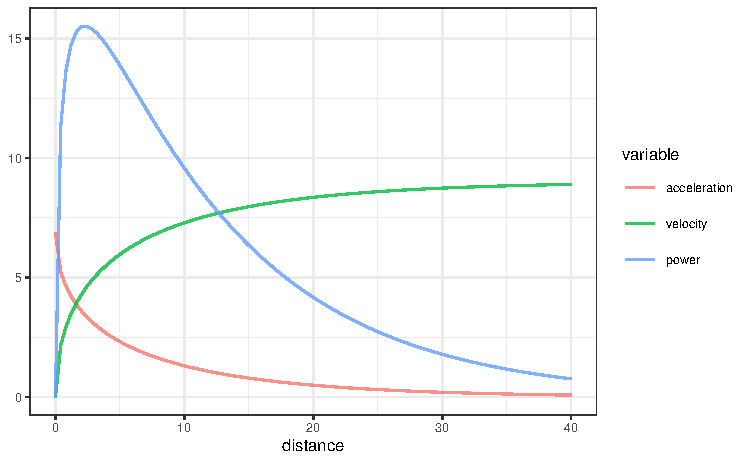
\includegraphics[width=0.9\linewidth]{paper_files/figure-latex/unnamed-chunk-2-1} \end{center}

\normalsize

Once we have estimated MSS and TAU, we can use \texttt{predict\_XXX()} family of functions to predict various relationships (i.e., time at distance, acceleration at distance, velocity at time, etc.):

\small

\begin{Shaded}
\begin{Highlighting}[]
\CommentTok{\# Predict time at distance}
\FunctionTok{predict\_time\_at\_distance}\NormalTok{(}
  \AttributeTok{distance =}\NormalTok{ split\_distance,}
  \AttributeTok{MSS =}\NormalTok{ m1}\SpecialCharTok{$}\NormalTok{parameters}\SpecialCharTok{$}\NormalTok{MSS,}
  \AttributeTok{TAU =}\NormalTok{ m1}\SpecialCharTok{$}\NormalTok{parameters}\SpecialCharTok{$}\NormalTok{TAU}
\NormalTok{)}
\CommentTok{\#\textgreater{} [1] 2.17 3.43 4.60 5.73}
\end{Highlighting}
\end{Shaded}

\normalsize

\hypertarget{air-resistance-and-the-calculation-of-force-and-mechanical-power}{%
\subsubsection{Air resistance and the calculation of force and mechanical power}\label{air-resistance-and-the-calculation-of-force-and-mechanical-power}}

To estimate force production at distance or time (using \texttt{predict\_force\_at\_distance()} and \texttt{predict\_force\_at\_time()} functions), as well as power production (using \texttt{predict\_power\_at\_distance()} and \texttt{predict\_power\_at\_time()} functions), one needs to take into account the air resistance. Air resistance (N) is estimated using \texttt{get\_air\_resistance()} function, which takes velocity, body mass (kg), body height (m), barometric pressure (Torr), air temperature (\(C^\circ\)), and wind velocity (\(ms^-1\)) as parameters (please refer to \protect\hyperlink{ref-arsacModelingEnergetics100m2002}{Arsac and Locatelli} (\protect\hyperlink{ref-arsacModelingEnergetics100m2002}{2002}), \protect\hyperlink{ref-samozinoSimpleMethodMeasuring2016}{Samozino et al.} (\protect\hyperlink{ref-samozinoSimpleMethodMeasuring2016}{2016}), and \protect\hyperlink{ref-vaningenschenauCanCyclePower1991}{van Ingen Schenau, Jacobs, and de Koning} (\protect\hyperlink{ref-vaningenschenauCanCyclePower1991}{1991}) for more information):

\small

\begin{Shaded}
\begin{Highlighting}[]
\FunctionTok{get\_air\_resistance}\NormalTok{(}
  \AttributeTok{velocity =} \DecValTok{5}\NormalTok{,}
  \AttributeTok{bodymass =} \DecValTok{80}\NormalTok{,}
  \AttributeTok{bodyheight =} \FloatTok{1.85}\NormalTok{,}
  \AttributeTok{barometric\_pressure =} \DecValTok{780}\NormalTok{,}
  \AttributeTok{air\_temperature =} \DecValTok{20}\NormalTok{,}
  \AttributeTok{wind\_velocity =} \FloatTok{0.5}
\NormalTok{)}
\CommentTok{\#\textgreater{} [1] 6.1}
\end{Highlighting}
\end{Shaded}

\normalsize

When estimating force and power, the air resistance parameters can be set using \texttt{"..."}, which are forwarded to the \texttt{get\_air\_resistance()}:

\small

\begin{Shaded}
\begin{Highlighting}[]
\CommentTok{\# To calculate horizontal force produced}
\FunctionTok{predict\_force\_at\_distance}\NormalTok{(}
  \AttributeTok{distance =}\NormalTok{ split\_distance,}
  \AttributeTok{MSS =}\NormalTok{ m1}\SpecialCharTok{$}\NormalTok{parameters}\SpecialCharTok{$}\NormalTok{MSS,}
  \AttributeTok{TAU =}\NormalTok{ m1}\SpecialCharTok{$}\NormalTok{parameters}\SpecialCharTok{$}\NormalTok{TAU,}
  \CommentTok{\# Additional parameters forwarded to get\_air\_resistance}
  \CommentTok{\# Otherwise, defaults are used}
  \AttributeTok{bodymass =} \DecValTok{80}\NormalTok{,}
  \AttributeTok{bodyheight =} \FloatTok{1.85}\NormalTok{,}
  \AttributeTok{barometric\_pressure =} \DecValTok{780}\NormalTok{,}
  \AttributeTok{air\_temperature =} \DecValTok{20}\NormalTok{,}
  \AttributeTok{wind\_velocity =} \FloatTok{0.5}
\NormalTok{)}
\CommentTok{\#\textgreater{} [1] 119.0  58.6  36.9  28.2}
\end{Highlighting}
\end{Shaded}

\normalsize

The easiest way to get all kinematics and kinetics for short sprints is to use \texttt{predict\_kinematics()} function:

\small

\begin{Shaded}
\begin{Highlighting}[]
\NormalTok{df }\OtherTok{\textless{}{-}} \FunctionTok{predict\_kinematics}\NormalTok{(}
\NormalTok{  m1,}
  \AttributeTok{max\_time =} \DecValTok{6}\NormalTok{,}
  \AttributeTok{frequency =} \DecValTok{100}\NormalTok{,}
  \CommentTok{\# Additional parameters forwarded to get\_air\_resistance}
  \CommentTok{\# Otherwise, defaults are used}
  \AttributeTok{bodymass =} \DecValTok{80}\NormalTok{,}
  \AttributeTok{bodyheight =} \FloatTok{1.85}\NormalTok{,}
  \AttributeTok{barometric\_pressure =} \DecValTok{780}\NormalTok{,}
  \AttributeTok{air\_temperature =} \DecValTok{20}\NormalTok{,}
  \AttributeTok{wind\_velocity =} \FloatTok{0.5}
\NormalTok{)}
\end{Highlighting}
\end{Shaded}

\normalsize

Plotting the model predictions can be done once we convert data from wide to long with the help of \textbf{ggplot2} (\protect\hyperlink{ref-R-ggplot2}{Wickham, Chang, et al. 2021}), \textbf{dplyr} (\protect\hyperlink{ref-R-dplyr}{Wickham, François, et al. 2021}), \textbf{tidyr} (\protect\hyperlink{ref-R-tidyr}{Wickham 2021a}), and \textbf{tidyverse} (\protect\hyperlink{ref-R-tidyverse}{Wickham 2021b}) packages:

\small

\begin{Shaded}
\begin{Highlighting}[]
\FunctionTok{require}\NormalTok{(tidyverse)}

\NormalTok{variable\_names }\OtherTok{\textless{}{-}} \FunctionTok{colnames}\NormalTok{(df)}

\NormalTok{df }\OtherTok{\textless{}{-}} \FunctionTok{pivot\_longer}\NormalTok{(}\AttributeTok{data =}\NormalTok{ df, }\AttributeTok{cols =} \SpecialCharTok{{-}}\DecValTok{2}\NormalTok{) }\SpecialCharTok{\%\textgreater{}\%}
  \FunctionTok{mutate}\NormalTok{(}\AttributeTok{name =} \FunctionTok{factor}\NormalTok{(name, }\AttributeTok{levels =}\NormalTok{ variable\_names))}

\FunctionTok{ggplot}\NormalTok{(df, }\FunctionTok{aes}\NormalTok{(}\AttributeTok{x =}\NormalTok{ distance, }\AttributeTok{y =}\NormalTok{ value)) }\SpecialCharTok{+}
  \FunctionTok{theme\_bw}\NormalTok{(}\DecValTok{8}\NormalTok{) }\SpecialCharTok{+}
  \FunctionTok{facet\_wrap}\NormalTok{(}\SpecialCharTok{\textasciitilde{}}\NormalTok{name, }\AttributeTok{scales =} \StringTok{"free\_y"}\NormalTok{) }\SpecialCharTok{+}
  \FunctionTok{geom\_line}\NormalTok{(}\AttributeTok{alpha =} \FloatTok{0.7}\NormalTok{) }\SpecialCharTok{+}
  \FunctionTok{ylab}\NormalTok{(}\ConstantTok{NULL}\NormalTok{) }\SpecialCharTok{+}
  \FunctionTok{xlab}\NormalTok{(}\StringTok{"Distance (m)"}\NormalTok{)}
\end{Highlighting}
\end{Shaded}

\begin{center}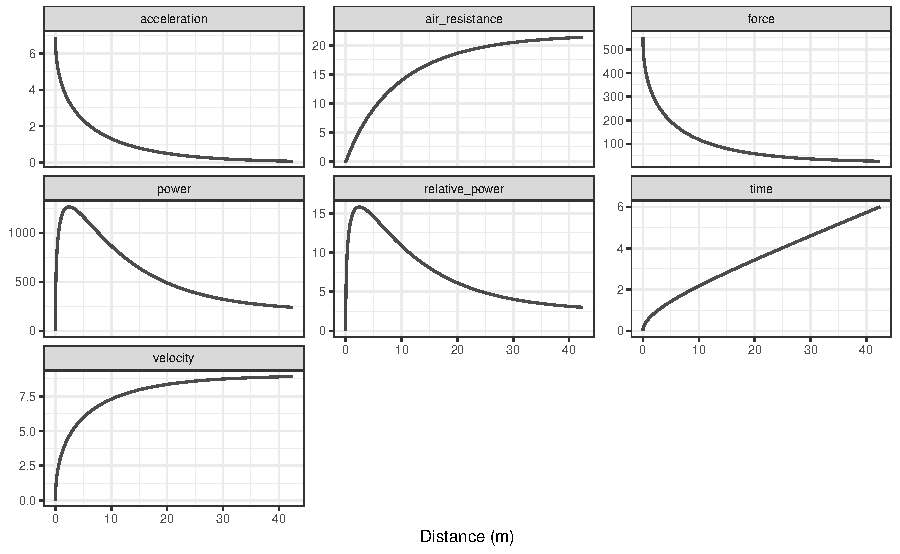
\includegraphics[width=0.9\linewidth]{paper_files/figure-latex/unnamed-chunk-7-1} \end{center}

\normalsize

These kinematic and kinetic variables are utilized in \protect\hyperlink{force-velocity-profile}{Force-Velocity profile} estimation, which is covered later in this paper.

\hypertarget{utility-functions}{%
\subsubsection{Utility functions}\label{utility-functions}}

Another valuable addition for sport scientists and coaches is the ability to determine the distances and times where 90\% of maximum sprinting speed is reached, or where peak power is within 90\% range. To identify these values, \textbf{shorts} package comes with \texttt{find\_XXX()} family of functions:

\small

\begin{Shaded}
\begin{Highlighting}[]
\CommentTok{\# Finds distance where 90\% of maximum sprinting speed is reached}
\FunctionTok{find\_velocity\_critical\_distance}\NormalTok{(}
  \AttributeTok{MSS =}\NormalTok{ m1}\SpecialCharTok{$}\NormalTok{parameters}\SpecialCharTok{$}\NormalTok{MSS,}
  \AttributeTok{TAU =}\NormalTok{ m1}\SpecialCharTok{$}\NormalTok{parameters}\SpecialCharTok{$}\NormalTok{TAU,}
  \AttributeTok{percent =} \FloatTok{0.9}
\NormalTok{)}
\CommentTok{\#\textgreater{} [1] 16.5}

\CommentTok{\# Finds maximal power and distance (this time using air resistance)}
\FunctionTok{find\_max\_power\_distance}\NormalTok{(}
  \AttributeTok{MSS =}\NormalTok{ m1}\SpecialCharTok{$}\NormalTok{parameters}\SpecialCharTok{$}\NormalTok{MSS,}
  \AttributeTok{TAU =}\NormalTok{ m1}\SpecialCharTok{$}\NormalTok{parameters}\SpecialCharTok{$}\NormalTok{TAU,}
  \CommentTok{\# Additional parameters forwarded to get\_air\_resistance}
  \CommentTok{\# Otherwise, defaults are used}
  \AttributeTok{bodymass =} \DecValTok{80}\NormalTok{,}
  \AttributeTok{bodyheight =} \FloatTok{1.85}\NormalTok{,}
  \AttributeTok{barometric\_pressure =} \DecValTok{780}\NormalTok{,}
  \AttributeTok{air\_temperature =} \DecValTok{20}\NormalTok{,}
  \AttributeTok{wind\_velocity =} \FloatTok{0.5}
\NormalTok{)}
\CommentTok{\#\textgreater{} $max\_power}
\CommentTok{\#\textgreater{} [1] 1264}
\CommentTok{\#\textgreater{} }
\CommentTok{\#\textgreater{} $distance}
\CommentTok{\#\textgreater{} [1] 2.46}

\CommentTok{\# Finds distance over 90\% power range}
\FunctionTok{find\_power\_critical\_distance}\NormalTok{(}
  \AttributeTok{MSS =}\NormalTok{ m1}\SpecialCharTok{$}\NormalTok{parameters}\SpecialCharTok{$}\NormalTok{MSS,}
  \AttributeTok{TAU =}\NormalTok{ m1}\SpecialCharTok{$}\NormalTok{parameters}\SpecialCharTok{$}\NormalTok{TAU,}
  \CommentTok{\# Additional parameters forwarded to get\_air\_resistance}
  \CommentTok{\# Otherwise, defaults are used}
  \AttributeTok{bodymass =} \DecValTok{80}\NormalTok{,}
  \AttributeTok{bodyheight =} \FloatTok{1.85}\NormalTok{,}
  \AttributeTok{barometric\_pressure =} \DecValTok{780}\NormalTok{,}
  \AttributeTok{air\_temperature =} \DecValTok{20}\NormalTok{,}
  \AttributeTok{wind\_velocity =} \FloatTok{0.5}
\NormalTok{)}
\CommentTok{\#\textgreater{} $lower}
\CommentTok{\#\textgreater{} [1] 0.959}
\CommentTok{\#\textgreater{} }
\CommentTok{\#\textgreater{} $upper}
\CommentTok{\#\textgreater{} [1] 5.44}
\end{Highlighting}
\end{Shaded}

\normalsize

\hypertarget{mixed-effects-model}{%
\subsubsection{Mixed-effects model}\label{mixed-effects-model}}

Sprint performance is often evaluated with a group of athletes (e.g., soccer club) representing a single strata of interest. Sports scientists can estimate individual profiles, or utilize mixed-effects models. To perform mixed-effects models in \textbf{shorts} for split times, one can use \texttt{mixed\_model\_using\_splits()} function. To demonstrate this functionality, we load the \texttt{split\_times} dataset provided in the \textbf{shorts} package:

\small

\begin{Shaded}
\begin{Highlighting}[]
\FunctionTok{data}\NormalTok{(split\_times)}

\CommentTok{\# Mixed model}
\NormalTok{m2 }\OtherTok{\textless{}{-}} \FunctionTok{mixed\_model\_using\_splits}\NormalTok{(}
  \AttributeTok{data =}\NormalTok{ split\_times,}
  \AttributeTok{distance =} \StringTok{"distance"}\NormalTok{,}
  \AttributeTok{time =} \StringTok{"time"}\NormalTok{,}
  \AttributeTok{athlete =} \StringTok{"athlete"}\NormalTok{,}

  \CommentTok{\# Select random effects}
  \CommentTok{\# Default is MSS and TAU}
  \AttributeTok{random =}\NormalTok{ MSS }\SpecialCharTok{+}\NormalTok{ TAU }\SpecialCharTok{\textasciitilde{}} \DecValTok{1}
\NormalTok{)}

\NormalTok{m2}
\CommentTok{\#\textgreater{} Estimated fixed model parameters}
\CommentTok{\#\textgreater{} {-}{-}{-}{-}{-}{-}{-}{-}{-}{-}{-}{-}{-}{-}{-}{-}{-}{-}{-}{-}{-}{-}{-}{-}{-}{-}{-}{-}{-}{-}{-}{-}}
\CommentTok{\#\textgreater{}                 MSS                 TAU                 MAC }
\CommentTok{\#\textgreater{}               8.065               0.655              12.309 }
\CommentTok{\#\textgreater{}                PMAX     time\_correction distance\_correction }
\CommentTok{\#\textgreater{}              24.818               0.000               0.000 }
\CommentTok{\#\textgreater{} }
\CommentTok{\#\textgreater{} Estimated random model parameters}
\CommentTok{\#\textgreater{} {-}{-}{-}{-}{-}{-}{-}{-}{-}{-}{-}{-}{-}{-}{-}{-}{-}{-}{-}{-}{-}{-}{-}{-}{-}{-}{-}{-}{-}{-}{-}{-}{-}}
\CommentTok{\#\textgreater{}     athlete  MSS   TAU  MAC PMAX time\_correction}
\CommentTok{\#\textgreater{} 1     James 9.69 0.847 11.4 27.7               0}
\CommentTok{\#\textgreater{} 2       Jim 7.83 0.505 15.5 30.4               0}
\CommentTok{\#\textgreater{} 3      John 7.78 0.727 10.7 20.8               0}
\CommentTok{\#\textgreater{} 4 Kimberley 8.57 0.802 10.7 22.9               0}
\CommentTok{\#\textgreater{} 5  Samantha 6.45 0.395 16.3 26.4               0}
\CommentTok{\#\textgreater{}   distance\_correction}
\CommentTok{\#\textgreater{} 1                   0}
\CommentTok{\#\textgreater{} 2                   0}
\CommentTok{\#\textgreater{} 3                   0}
\CommentTok{\#\textgreater{} 4                   0}
\CommentTok{\#\textgreater{} 5                   0}
\CommentTok{\#\textgreater{} }
\CommentTok{\#\textgreater{} Model fit estimators}
\CommentTok{\#\textgreater{} {-}{-}{-}{-}{-}{-}{-}{-}{-}{-}{-}{-}{-}{-}{-}{-}{-}{-}{-}{-}}
\CommentTok{\#\textgreater{}       RSE R\_squared    minErr    maxErr maxAbsErr      RMSE }
\CommentTok{\#\textgreater{}    0.0260    0.9998   {-}0.0496    0.0293    0.0496    0.0214 }
\CommentTok{\#\textgreater{}       MAE      MAPE }
\CommentTok{\#\textgreater{}    0.0172    0.9019}
\end{Highlighting}
\end{Shaded}

\normalsize

Additional information about mixed-effects model performed using the \texttt{nlme} package (\protect\hyperlink{ref-R-nlme}{Pinheiro, Bates, and R-core 2021}) can be obtained using \texttt{summary()} function. S3 method \texttt{coef()} when applied on mixed-model result will return both the fixed and random effects.

To create a simple plot of the model, use S3 \texttt{plot()} method.

\small

\begin{Shaded}
\begin{Highlighting}[]
\FunctionTok{plot}\NormalTok{(m2) }\SpecialCharTok{+} \FunctionTok{theme\_bw}\NormalTok{(}\DecValTok{8}\NormalTok{)}
\end{Highlighting}
\end{Shaded}

\begin{center}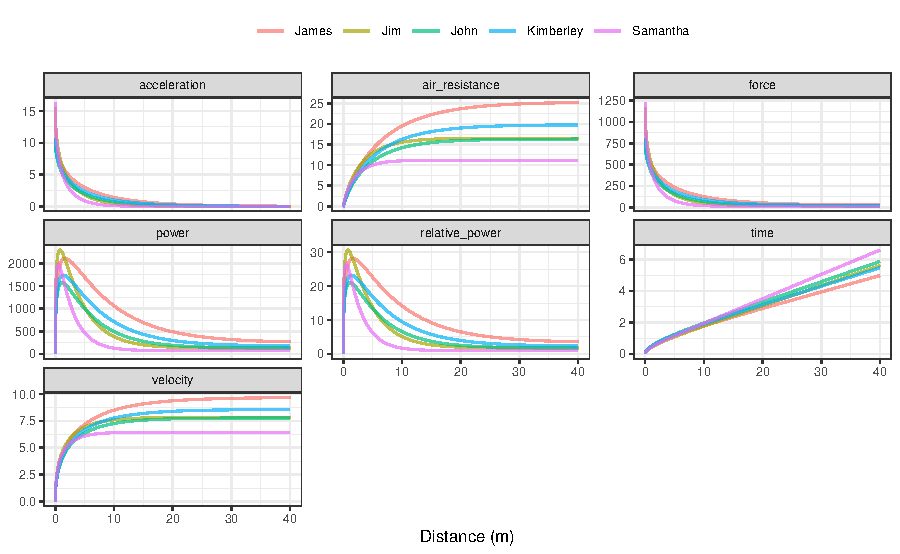
\includegraphics[width=0.9\linewidth]{paper_files/figure-latex/unnamed-chunk-11-1} \end{center}

\normalsize

The following figure contains kinematics for all athletes in \texttt{split\_times} dataset. Please note that power calculation takes default parameters for each individual:

\small

\begin{Shaded}
\begin{Highlighting}[]
\NormalTok{df }\OtherTok{\textless{}{-}} \FunctionTok{predict\_kinematics}\NormalTok{(m2, }\AttributeTok{max\_time =} \DecValTok{10}\NormalTok{)}

\NormalTok{variable\_names }\OtherTok{\textless{}{-}} \FunctionTok{colnames}\NormalTok{(df)}

\NormalTok{df }\OtherTok{\textless{}{-}} \FunctionTok{pivot\_longer}\NormalTok{(df, }\AttributeTok{cols =} \FunctionTok{c}\NormalTok{(}\SpecialCharTok{{-}}\DecValTok{1}\NormalTok{, }\SpecialCharTok{{-}}\DecValTok{3}\NormalTok{)) }\SpecialCharTok{\%\textgreater{}\%}
  \FunctionTok{mutate}\NormalTok{(}\AttributeTok{name =} \FunctionTok{factor}\NormalTok{(name, }\AttributeTok{levels =}\NormalTok{ variable\_names))}

\FunctionTok{ggplot}\NormalTok{(}
  \FunctionTok{filter}\NormalTok{(df, distance }\SpecialCharTok{\textless{}} \DecValTok{40}\NormalTok{),}
  \FunctionTok{aes}\NormalTok{(}\AttributeTok{x =}\NormalTok{ distance, }\AttributeTok{y =}\NormalTok{ value, }\AttributeTok{group =}\NormalTok{ athlete, }\AttributeTok{color =}\NormalTok{ athlete)}
\NormalTok{) }\SpecialCharTok{+}
  \FunctionTok{theme\_bw}\NormalTok{(}\DecValTok{8}\NormalTok{) }\SpecialCharTok{+}
  \FunctionTok{facet\_wrap}\NormalTok{(}\SpecialCharTok{\textasciitilde{}}\NormalTok{name, }\AttributeTok{scales =} \StringTok{"free\_y"}\NormalTok{) }\SpecialCharTok{+}
  \FunctionTok{geom\_line}\NormalTok{(}\AttributeTok{alpha =} \FloatTok{0.7}\NormalTok{) }\SpecialCharTok{+}
  \FunctionTok{ylab}\NormalTok{(}\ConstantTok{NULL}\NormalTok{) }\SpecialCharTok{+}
  \FunctionTok{xlab}\NormalTok{(}\StringTok{"Distance (m)"}\NormalTok{) }\SpecialCharTok{+}
  \FunctionTok{theme}\NormalTok{(}
    \AttributeTok{legend.position =} \StringTok{"top"}\NormalTok{,}
    \AttributeTok{legend.title =} \FunctionTok{element\_blank}\NormalTok{()}
\NormalTok{  )}
\end{Highlighting}
\end{Shaded}

\begin{center}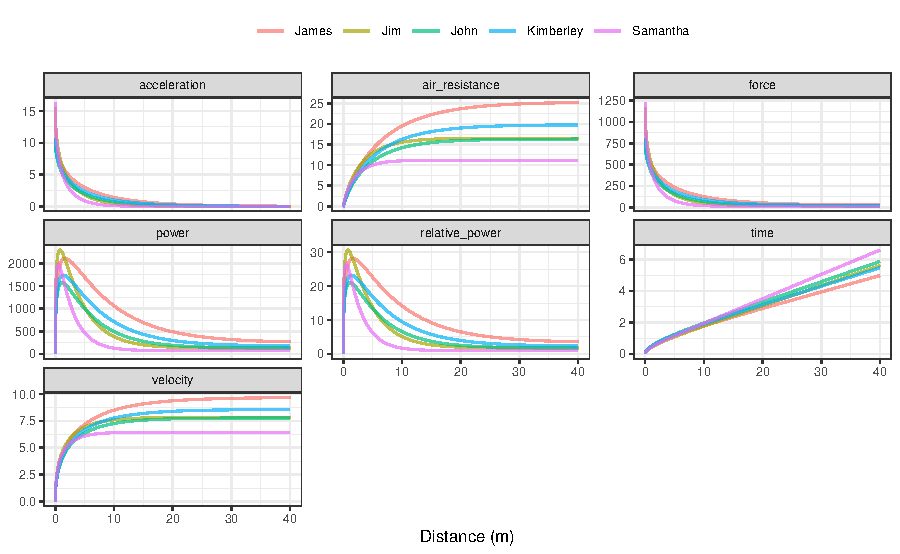
\includegraphics[width=0.9\linewidth]{paper_files/figure-latex/unnamed-chunk-12-1} \end{center}

\normalsize

\hypertarget{estimating-short-sprint-parameters-using-radar-gun}{%
\subsection{Estimating short sprint parameters using radar gun}\label{estimating-short-sprint-parameters-using-radar-gun}}

Estimation of the short sprint profile using radar gun data takes time as predictor and velocity as the outcome variable. Thus equation \eqref{eq:velocity-time} is used to estimate MSS and TAU.

Let's consider the same example of an athlete with MSS equal to 9 \(ms^{-1}\), TAU equal to 1.3, and MAC equal to 6.92 \(ms^{-2}\) performing 40m sprint with velocity estimated using radar run (in this case with 1 Hz sampling rate).

\small

\begin{Shaded}
\begin{Highlighting}[]
\NormalTok{sprint\_time }\OtherTok{\textless{}{-}} \FunctionTok{seq}\NormalTok{(}\DecValTok{0}\NormalTok{, }\DecValTok{6}\NormalTok{, }\DecValTok{1}\NormalTok{)}

\NormalTok{sprint\_velocity }\OtherTok{\textless{}{-}} \FunctionTok{c}\NormalTok{(}\FloatTok{0.00}\NormalTok{, }\FloatTok{4.83}\NormalTok{, }\FloatTok{7.07}\NormalTok{, }\FloatTok{8.10}\NormalTok{, }\FloatTok{8.59}\NormalTok{, }\FloatTok{8.81}\NormalTok{, }\FloatTok{8.91}\NormalTok{)}

\NormalTok{m3 }\OtherTok{\textless{}{-}} \FunctionTok{model\_using\_radar}\NormalTok{(}
  \AttributeTok{velocity =}\NormalTok{ sprint\_velocity,}
  \AttributeTok{time =}\NormalTok{ sprint\_time}
\NormalTok{)}
\end{Highlighting}
\end{Shaded}

\normalsize

Both split and radar gun models allow the use of \emph{weighted} non-linear regression. For example, we can give more weight to shorter distance or faster velocities. Weighted non-linear regression is performed by setting \texttt{weights} parameter:

\small

\begin{Shaded}
\begin{Highlighting}[]
\NormalTok{m3\_weighted }\OtherTok{\textless{}{-}} \FunctionTok{model\_using\_radar}\NormalTok{(}
  \AttributeTok{velocity =}\NormalTok{ sprint\_velocity,}
  \AttributeTok{time =}\NormalTok{ sprint\_time,}
  \AttributeTok{weights =} \DecValTok{1} \SpecialCharTok{/}\NormalTok{ (sprint\_velocity }\SpecialCharTok{+} \DecValTok{1}\NormalTok{)}
\NormalTok{)}
\end{Highlighting}
\end{Shaded}

\normalsize

\hypertarget{mixed-effects-model-1}{%
\subsubsection{Mixed-effects model}\label{mixed-effects-model-1}}

Mixed-effects model using radar data is done using \texttt{mixed\_model\_using\_radar()} function. To perform mixed model, let's load data that comes with \textbf{shorts} package.

\small

\begin{Shaded}
\begin{Highlighting}[]
\FunctionTok{data}\NormalTok{(}\StringTok{"radar\_gun\_data"}\NormalTok{)}

\NormalTok{m4 }\OtherTok{\textless{}{-}} \FunctionTok{mixed\_model\_using\_radar}\NormalTok{(}
\NormalTok{  radar\_gun\_data,}
  \AttributeTok{time =} \StringTok{"time"}\NormalTok{,}
  \AttributeTok{velocity =} \StringTok{"velocity"}\NormalTok{,}
  \AttributeTok{athlete =} \StringTok{"athlete"}
\NormalTok{)}
\end{Highlighting}
\end{Shaded}

\normalsize

\hypertarget{force-velocity-profile}{%
\subsection{Force-Velocity profile}\label{force-velocity-profile}}

To create \emph{Force-Velocity Profile} (FVP) using single athlete estimated sprint model parameters (i.e., TAU and MSS), you can use \texttt{get\_FV\_profile()} function. When estimating FVP, athlete body mass (kg) can be set using \texttt{bodymass} parameter, while the air resistance parameters can be set using \texttt{"..."}, which are forwarded to the \texttt{get\_air\_resistance()} function. Details of the FVP method implemented in the \textbf{shorts} package, as well as the interpretation from a sprint training perspective, are covered elsewhere (\protect\hyperlink{ref-haugenPowerForceVelocityProfilingSprinting2020}{Thomas A. Haugen, Breitschädel, and Samozino 2020}; \protect\hyperlink{ref-morinInterpretingPowerForceVelocityProfiles2016}{Jean-Benoit Morin and Samozino 2016}; \protect\hyperlink{ref-morinSimpleMethodComputing2019}{Jean-Benoit Morin et al. 2019}; \protect\hyperlink{ref-samozinoSimpleMethodMeasuring2016}{Samozino et al. 2016}).

\small

\begin{Shaded}
\begin{Highlighting}[]
\CommentTok{\# To create Force{-}Velocity Profile}
\NormalTok{fvp }\OtherTok{\textless{}{-}} \FunctionTok{get\_FV\_profile}\NormalTok{(}
  \AttributeTok{MSS =}\NormalTok{ m1}\SpecialCharTok{$}\NormalTok{parameters}\SpecialCharTok{$}\NormalTok{MSS,}
  \AttributeTok{TAU =}\NormalTok{ m1}\SpecialCharTok{$}\NormalTok{parameters}\SpecialCharTok{$}\NormalTok{TAU,}
  \AttributeTok{bodymass =} \DecValTok{80}\NormalTok{,}
  \CommentTok{\# Additional parameters forwarded to get\_air\_resistance}
  \CommentTok{\# Otherwise, defaults are used}
  \AttributeTok{bodyheight =} \FloatTok{1.85}\NormalTok{,}
  \AttributeTok{barometric\_pressure =} \DecValTok{780}\NormalTok{,}
  \AttributeTok{air\_temperature =} \DecValTok{20}\NormalTok{,}
  \AttributeTok{wind\_velocity =} \FloatTok{0.5}
\NormalTok{)}

\NormalTok{fvp}
\CommentTok{\#\textgreater{} Estimated Force{-}Velocity Profile}
\CommentTok{\#\textgreater{} {-}{-}{-}{-}{-}{-}{-}{-}{-}{-}{-}{-}{-}{-}{-}{-}{-}{-}{-}{-}{-}{-}{-}{-}{-}{-}{-}{-}{-}{-}{-}{-}}
\CommentTok{\#\textgreater{}      bodymass            F0        F0\_rel            V0 }
\CommentTok{\#\textgreater{}      80.00000     544.51032       6.80638       9.36184 }
\CommentTok{\#\textgreater{}          Pmax Pmax\_relative      FV\_slope  RFmax\_cutoff }
\CommentTok{\#\textgreater{}    1274.40402      15.93005      {-}0.72703       0.30000 }
\CommentTok{\#\textgreater{}         RFmax           Drf        RSE\_FV       RSE\_Drf }
\CommentTok{\#\textgreater{}       0.48779      {-}0.06676       1.54814       0.00447}
\end{Highlighting}
\end{Shaded}

\normalsize

To plot FVP kinematics and kinetics (which are exactly the same as generated by the \texttt{predict\_kinematics()} function), use S3 \texttt{plot()} function. By default, FVP estimated kinetics are plotted against velocity (on x-axis).

\small

\begin{Shaded}
\begin{Highlighting}[]
\FunctionTok{plot}\NormalTok{(fvp) }\SpecialCharTok{+} \FunctionTok{theme\_bw}\NormalTok{(}\DecValTok{8}\NormalTok{)}
\end{Highlighting}
\end{Shaded}

\begin{center}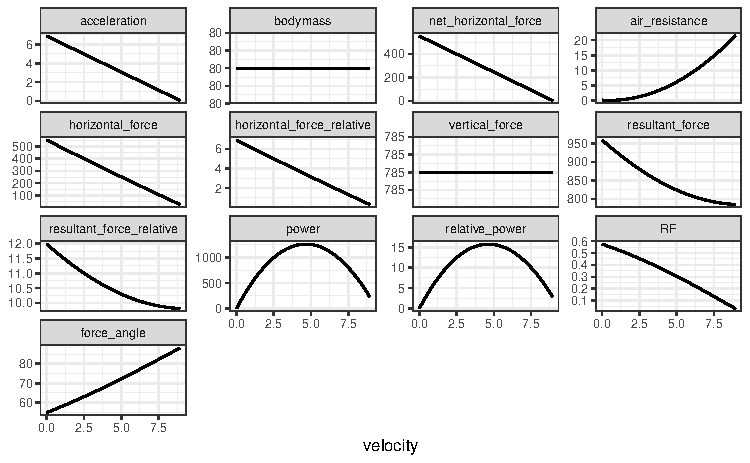
\includegraphics[width=0.9\linewidth]{paper_files/figure-latex/unnamed-chunk-17-1} \end{center}

\normalsize

To plot FVP estimated kinetics against time, use \texttt{type\ =\ "time"} parameter:

\small

\begin{Shaded}
\begin{Highlighting}[]
\FunctionTok{plot}\NormalTok{(fvp, }\StringTok{"time"}\NormalTok{) }\SpecialCharTok{+} \FunctionTok{theme\_bw}\NormalTok{(}\DecValTok{8}\NormalTok{)}
\end{Highlighting}
\end{Shaded}

\normalsize

\hypertarget{problems-with-estimation}{%
\section{Problems with estimation}\label{problems-with-estimation}}

There is a challenge when collecting sprint data that could have a substantial impact on modeled outcomes. To ensure accurate parameter outcomes, the initial force production must be synced with start time (\protect\hyperlink{ref-haugenPowerForceVelocityProfilingSprinting2020}{Thomas A. Haugen, Breitschädel, and Samozino 2020}; \protect\hyperlink{ref-haugenSprintMechanicalVariables2019}{Thomas A. Haugen, Breitschädel, and Seiler 2019}). Below we describe this challenge when using radar guns or timing gates and suggest potential solutions within the \textbf{shorts} package.

\hypertarget{problems-with-time-sync-with-radar-gun}{%
\subsection{Problems with time sync with radar gun}\label{problems-with-time-sync-with-radar-gun}}

One source of error in the modeled estimation using a radar gun is the time synchronization. In theory, synchronization is ideal when a sprint is initiated at \(t=0\) (i.e., \(v(t=0) = 0\)). In practice, this is often not the case. Let's use our athlete and add and deduct 0.5 s to simulate an error in synchronization and its effect on estimated MSS and TAU.

\small

\begin{Shaded}
\begin{Highlighting}[]
\NormalTok{df }\OtherTok{\textless{}{-}} \FunctionTok{tibble}\NormalTok{(}
  \StringTok{\textasciigrave{}}\AttributeTok{true time}\StringTok{\textasciigrave{}} \OtherTok{=}\NormalTok{ sprint\_time,}
  \AttributeTok{velocity =}\NormalTok{ sprint\_velocity,}
  \StringTok{\textasciigrave{}}\AttributeTok{0.5s added}\StringTok{\textasciigrave{}} \OtherTok{=} \StringTok{\textasciigrave{}}\AttributeTok{true time}\StringTok{\textasciigrave{}} \SpecialCharTok{+} \FloatTok{0.5}\NormalTok{,}
  \StringTok{\textasciigrave{}}\AttributeTok{0.5s deducted}\StringTok{\textasciigrave{}} \OtherTok{=} \StringTok{\textasciigrave{}}\AttributeTok{true time}\StringTok{\textasciigrave{}} \SpecialCharTok{{-}} \FloatTok{0.5}
\NormalTok{)}

\NormalTok{plot\_df }\OtherTok{\textless{}{-}} \FunctionTok{pivot\_longer}\NormalTok{(df, }\AttributeTok{cols =} \SpecialCharTok{{-}}\DecValTok{2}\NormalTok{, }\AttributeTok{names\_to =} \StringTok{"Sync issue"}\NormalTok{)}

\FunctionTok{ggplot}\NormalTok{(}
\NormalTok{  plot\_df,}
  \FunctionTok{aes}\NormalTok{(}\AttributeTok{x =}\NormalTok{ value, }\AttributeTok{y =}\NormalTok{ velocity, }\AttributeTok{color =} \StringTok{\textasciigrave{}}\AttributeTok{Sync issue}\StringTok{\textasciigrave{}}\NormalTok{)}
\NormalTok{) }\SpecialCharTok{+}
  \FunctionTok{theme\_bw}\NormalTok{(}\DecValTok{8}\NormalTok{) }\SpecialCharTok{+}
  \FunctionTok{geom\_line}\NormalTok{(}\AttributeTok{alpha =} \FloatTok{0.7}\NormalTok{) }\SpecialCharTok{+}
  \FunctionTok{xlab}\NormalTok{(}\StringTok{"Time (s)"}\NormalTok{) }\SpecialCharTok{+}
  \FunctionTok{ylab}\NormalTok{(}\FunctionTok{expression}\NormalTok{(}\StringTok{"Velocity ("} \SpecialCharTok{*}\NormalTok{ ms}\SpecialCharTok{\^{}{-}}\DecValTok{1} \SpecialCharTok{*} \StringTok{")"}\NormalTok{)) }\SpecialCharTok{+}
  \FunctionTok{theme}\NormalTok{(}
    \AttributeTok{legend.title =} \FunctionTok{element\_blank}\NormalTok{(),}
    \AttributeTok{legend.position =} \StringTok{"top"}
\NormalTok{  )}
\end{Highlighting}
\end{Shaded}

\begin{center}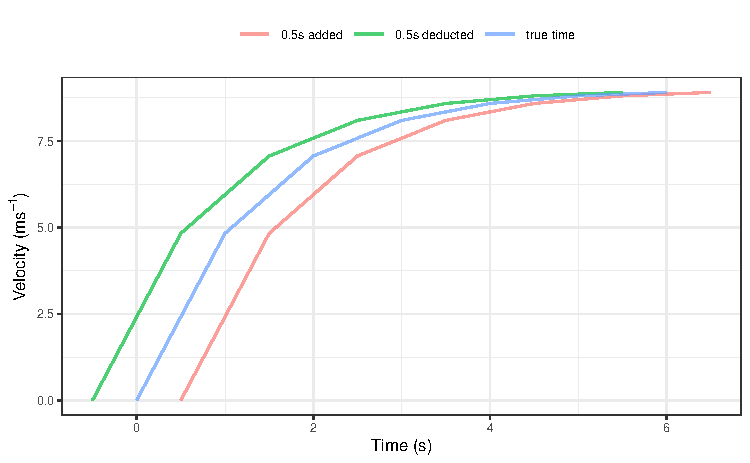
\includegraphics[width=0.9\linewidth]{paper_files/figure-latex/unnamed-chunk-19-1} \end{center}

\normalsize

The following three models estimate MSS and TAU from the three datasets. Tables are created using the \texttt{kable()} function from the \textbf{knitr} package (\protect\hyperlink{ref-knitr2014}{Xie 2014}, \protect\hyperlink{ref-knitr2015}{2015}, \protect\hyperlink{ref-R-knitr}{2021b}) and \texttt{kable\_styling()} function from the \textbf{kableExtra} package (\protect\hyperlink{ref-R-kableExtra}{Zhu 2021}).

\small

\begin{Shaded}
\begin{Highlighting}[]
\FunctionTok{require}\NormalTok{(knitr)}
\FunctionTok{require}\NormalTok{(kableExtra)}

\CommentTok{\# Without synchronization issues}
\NormalTok{m5 }\OtherTok{\textless{}{-}} \FunctionTok{model\_using\_radar}\NormalTok{(}
  \AttributeTok{velocity =}\NormalTok{ df}\SpecialCharTok{$}\NormalTok{velocity,}
  \AttributeTok{time =}\NormalTok{ df}\SpecialCharTok{$}\StringTok{\textasciigrave{}}\AttributeTok{true time}\StringTok{\textasciigrave{}}
\NormalTok{)}

\CommentTok{\# With time added}
\NormalTok{m6 }\OtherTok{\textless{}{-}} \FunctionTok{model\_using\_radar}\NormalTok{(}
  \AttributeTok{velocity =}\NormalTok{ df}\SpecialCharTok{$}\NormalTok{velocity,}
  \AttributeTok{time =}\NormalTok{ df}\SpecialCharTok{$}\StringTok{\textasciigrave{}}\AttributeTok{0.5s added}\StringTok{\textasciigrave{}}
\NormalTok{)}

\CommentTok{\# With time deducted}
\NormalTok{m7 }\OtherTok{\textless{}{-}} \FunctionTok{model\_using\_radar}\NormalTok{(}
  \AttributeTok{velocity =}\NormalTok{ df}\SpecialCharTok{$}\NormalTok{velocity,}
  \AttributeTok{time =}\NormalTok{ df}\SpecialCharTok{$}\StringTok{\textasciigrave{}}\AttributeTok{0.5s deducted}\StringTok{\textasciigrave{}}
\NormalTok{)}

\NormalTok{model\_df }\OtherTok{\textless{}{-}} \FunctionTok{rbind}\NormalTok{(}
  \FunctionTok{data.frame}\NormalTok{(}
    \AttributeTok{model =} \StringTok{"True time"}\NormalTok{,}
    \FunctionTok{t}\NormalTok{(}\FunctionTok{coef}\NormalTok{(m5))}
\NormalTok{  ),}
  \FunctionTok{data.frame}\NormalTok{(}
    \AttributeTok{model =} \StringTok{"Added 0.5s time"}\NormalTok{,}
    \FunctionTok{t}\NormalTok{(}\FunctionTok{coef}\NormalTok{(m6))}
\NormalTok{  ),}
  \FunctionTok{data.frame}\NormalTok{(}
    \AttributeTok{model =} \StringTok{"Deducted 0.5s time"}\NormalTok{,}
    \FunctionTok{t}\NormalTok{(}\FunctionTok{coef}\NormalTok{(m7))}
\NormalTok{  )}
\NormalTok{)}

\FunctionTok{kable}\NormalTok{(model\_df, }\AttributeTok{digits =} \DecValTok{2}\NormalTok{, }\AttributeTok{booktabs =} \ConstantTok{TRUE}\NormalTok{)}
\end{Highlighting}
\end{Shaded}

\begin{tabular}{lrrrrrr}
\toprule
model & MSS & TAU & MAC & PMAX & time\_correction & distance\_correction\\
\midrule
True time & 9.00 & 1.30 & 6.92 & 15.6 & 0 & 0\\
Added 0.5s time & 9.91 & 2.34 & 4.23 & 10.5 & 0 & 0\\
Deducted 0.5s time & 10.08 & 1.86 & 5.43 & 13.7 & 0 & 0\\
\bottomrule
\end{tabular}

\normalsize

As can be seen from the example, all estimated parameters are affected by an error in synchronization of time with velocity (with MSS being the least affected in this example). The potential solution incorporated into the \textbf{shorts} package involves estimation of the \emph{time correction} parameter using the following equation:

\begin{equation}
  v(t) = MSS \times (1 - e^{-\frac{t + time \; correction}{TAU}}) \label{eq:velocity-time-correction}
\end{equation}

This model is incorporated in the \texttt{model\_using\_radar\_with\_time\_correction()} function:

\small

\begin{Shaded}
\begin{Highlighting}[]
\CommentTok{\# With time added}
\NormalTok{m8 }\OtherTok{\textless{}{-}} \FunctionTok{model\_using\_radar\_with\_time\_correction}\NormalTok{(}
  \AttributeTok{velocity =}\NormalTok{ df}\SpecialCharTok{$}\NormalTok{velocity,}
  \AttributeTok{time =}\NormalTok{ df}\SpecialCharTok{$}\StringTok{\textasciigrave{}}\AttributeTok{0.5s added}\StringTok{\textasciigrave{}}
\NormalTok{)}
\FunctionTok{coef}\NormalTok{(m8)}
\CommentTok{\#\textgreater{}                 MSS                 TAU                 MAC }
\CommentTok{\#\textgreater{}                9.00                1.30                6.92 }
\CommentTok{\#\textgreater{}                PMAX     time\_correction distance\_correction }
\CommentTok{\#\textgreater{}               15.58               {-}0.50                0.00}

\CommentTok{\# With time deducted}
\NormalTok{m9 }\OtherTok{\textless{}{-}} \FunctionTok{model\_using\_radar\_with\_time\_correction}\NormalTok{(}
  \AttributeTok{velocity =}\NormalTok{ df}\SpecialCharTok{$}\NormalTok{velocity,}
  \AttributeTok{time =}\NormalTok{ df}\SpecialCharTok{$}\StringTok{\textasciigrave{}}\AttributeTok{0.5s deducted}\StringTok{\textasciigrave{}}
\NormalTok{)}
\FunctionTok{coef}\NormalTok{(m9)}
\CommentTok{\#\textgreater{}                 MSS                 TAU                 MAC }
\CommentTok{\#\textgreater{}                9.00                1.30                6.92 }
\CommentTok{\#\textgreater{}                PMAX     time\_correction distance\_correction }
\CommentTok{\#\textgreater{}               15.58                0.50                0.00}
\end{Highlighting}
\end{Shaded}

\normalsize

When using \texttt{predict\_XXX()} family of functions, one can provide estimated time correction to get predictions at original time scale.

\small

\begin{Shaded}
\begin{Highlighting}[]
\CommentTok{\# Using the true time}
\FunctionTok{predict\_velocity\_at\_time}\NormalTok{(}
  \AttributeTok{time =}\NormalTok{ df}\SpecialCharTok{$}\StringTok{\textasciigrave{}}\AttributeTok{true time}\StringTok{\textasciigrave{}}\NormalTok{,}
  \AttributeTok{MSS =}\NormalTok{ m5}\SpecialCharTok{$}\NormalTok{parameters}\SpecialCharTok{$}\NormalTok{MSS,}
  \AttributeTok{TAU =}\NormalTok{ m5}\SpecialCharTok{$}\NormalTok{parameters}\SpecialCharTok{$}\NormalTok{TAU}
\NormalTok{)}
\CommentTok{\#\textgreater{} [1] 0.00 4.83 7.07 8.11 8.59 8.81 8.91}

\CommentTok{\# Using time with sync issues}
\FunctionTok{predict\_velocity\_at\_time}\NormalTok{(}
  \AttributeTok{time =}\NormalTok{ df}\SpecialCharTok{$}\StringTok{\textasciigrave{}}\AttributeTok{0.5s added}\StringTok{\textasciigrave{}}\NormalTok{,}
  \AttributeTok{MSS =}\NormalTok{ m8}\SpecialCharTok{$}\NormalTok{parameters}\SpecialCharTok{$}\NormalTok{MSS,}
  \AttributeTok{TAU =}\NormalTok{ m8}\SpecialCharTok{$}\NormalTok{parameters}\SpecialCharTok{$}\NormalTok{TAU,}
  \AttributeTok{time\_correction =}\NormalTok{ m8}\SpecialCharTok{$}\NormalTok{parameters}\SpecialCharTok{$}\NormalTok{time\_correction}
\NormalTok{)}
\CommentTok{\#\textgreater{} [1] 0.0000782 4.8299729 7.0681475 8.1053182 8.5859434 8.8086652}
\CommentTok{\#\textgreater{} [7] 8.9118746}
\end{Highlighting}
\end{Shaded}

\normalsize

\hypertarget{mixed-model-approach}{%
\subsubsection{Mixed-model approach}\label{mixed-model-approach}}

When it comes to mixed-model approach, time correction can be modeled as a fixed effect or random effect using the \texttt{mixed\_model\_using\_radar\_with\_time\_correction()} function.

\small

\begin{Shaded}
\begin{Highlighting}[]
\CommentTok{\# Adding 0.5s to radar\_gun\_data}
\NormalTok{radar\_gun\_data}\SpecialCharTok{$}\NormalTok{time }\OtherTok{\textless{}{-}}\NormalTok{ radar\_gun\_data}\SpecialCharTok{$}\NormalTok{time }\SpecialCharTok{+} \FloatTok{0.5}

\CommentTok{\# Mixed model with time correction being fixed effect}
\NormalTok{m10 }\OtherTok{\textless{}{-}} \FunctionTok{mixed\_model\_using\_radar\_with\_time\_correction}\NormalTok{(}
\NormalTok{  radar\_gun\_data,}
  \AttributeTok{time =} \StringTok{"time"}\NormalTok{,}
  \AttributeTok{velocity =} \StringTok{"velocity"}\NormalTok{,}
  \AttributeTok{athlete =} \StringTok{"athlete"}\NormalTok{,}
  \AttributeTok{random =}\NormalTok{ MSS }\SpecialCharTok{+}\NormalTok{ TAU }\SpecialCharTok{\textasciitilde{}} \DecValTok{1}
\NormalTok{)}

\CommentTok{\# Mixed model with time correction being random effect}
\NormalTok{m11 }\OtherTok{\textless{}{-}} \FunctionTok{mixed\_model\_using\_radar\_with\_time\_correction}\NormalTok{(}
\NormalTok{  radar\_gun\_data,}
  \AttributeTok{time =} \StringTok{"time"}\NormalTok{,}
  \AttributeTok{velocity =} \StringTok{"velocity"}\NormalTok{,}
  \AttributeTok{athlete =} \StringTok{"athlete"}\NormalTok{,}
  \AttributeTok{random =}\NormalTok{ MSS }\SpecialCharTok{+}\NormalTok{ TAU }\SpecialCharTok{+}\NormalTok{ time\_correction }\SpecialCharTok{\textasciitilde{}} \DecValTok{1}
\NormalTok{)}
\end{Highlighting}
\end{Shaded}

\normalsize

\hypertarget{problems-at-the-start-when-using-timing-gates}{%
\subsection{Problems at the start when using timing gates}\label{problems-at-the-start-when-using-timing-gates}}

Let's imagine we have two twin brothers with same short sprint characteristics: MSS equal to 9 \(ms^{-1}\), TAU equal to 1.3, and MAC equal to 6.92 \(ms^{-2}\). Let's call them John and Jack. They both perform 40m sprint using timing gates set at 5, 10, 20, 30, and 40 m. The initial timing gate at the start (i.e., \(d=0\) m) serves to activate the timing system (i.e., when they cross the beam).

John represents the \emph{theoretical model}, in which we assume that the initial force production and the timing initiation are perfectly synchronized. Jack, on the other hand, represents a \emph{practical model}, and decides to move slightly behind the initial timing gate (i.e.~for 0.5 m) and use body rocking to initiate the sprint start. In other words, Jack is using a \emph{flying start}, a common scenario when testing field sports athletes. Flying start distance is often recommended to avoid premature triggering of the timing system by lifted knees or swinging
arms (\protect\hyperlink{ref-altmannAccuracySingleBeam2018}{Altmann et al. 2018}, \protect\hyperlink{ref-altmannDifferentStartingDistances2015}{2015}, \protect\hyperlink{ref-altmannValiditySingleBeamTiming2017}{2017}; \protect\hyperlink{ref-haugenPowerForceVelocityProfilingSprinting2020}{Thomas A. Haugen, Breitschädel, and Samozino 2020}; \protect\hyperlink{ref-haugenSprintRunningPerformance2016}{T. Haugen and Buchheit 2016}).

\small

\begin{Shaded}
\begin{Highlighting}[]
\NormalTok{MSS }\OtherTok{\textless{}{-}} \DecValTok{9}
\NormalTok{TAU }\OtherTok{\textless{}{-}} \FloatTok{1.3}
\NormalTok{MAC }\OtherTok{\textless{}{-}}\NormalTok{ MSS }\SpecialCharTok{/}\NormalTok{ TAU}

\NormalTok{split\_times }\OtherTok{\textless{}{-}} \FunctionTok{tibble}\NormalTok{(}
  \AttributeTok{distance =} \FunctionTok{c}\NormalTok{(}\DecValTok{5}\NormalTok{, }\DecValTok{10}\NormalTok{, }\DecValTok{20}\NormalTok{, }\DecValTok{30}\NormalTok{, }\DecValTok{40}\NormalTok{),}
  \AttributeTok{john\_time =} \FunctionTok{predict\_time\_at\_distance}\NormalTok{(distance, MSS, TAU),}

  \CommentTok{\# Jack\textquotesingle{}s performance}
  \AttributeTok{jack\_distance =}\NormalTok{ distance }\SpecialCharTok{+} \FloatTok{0.5}\NormalTok{,}
  \AttributeTok{jack\_true\_time =} \FunctionTok{predict\_time\_at\_distance}\NormalTok{(jack\_distance, MSS, TAU),}
  \AttributeTok{time\_05m =} \FunctionTok{predict\_time\_at\_distance}\NormalTok{(}\FloatTok{0.5}\NormalTok{, MSS, TAU),}
  \AttributeTok{jack\_time =}\NormalTok{ jack\_true\_time }\SpecialCharTok{{-}}\NormalTok{ time\_05m}
\NormalTok{)}
\end{Highlighting}
\end{Shaded}

\normalsize

Here is a graphical representation of the sprint splits (please refer to the \protect\hyperlink{supplemental-material}{Supplemental material} for the R code):

\small

\begin{center}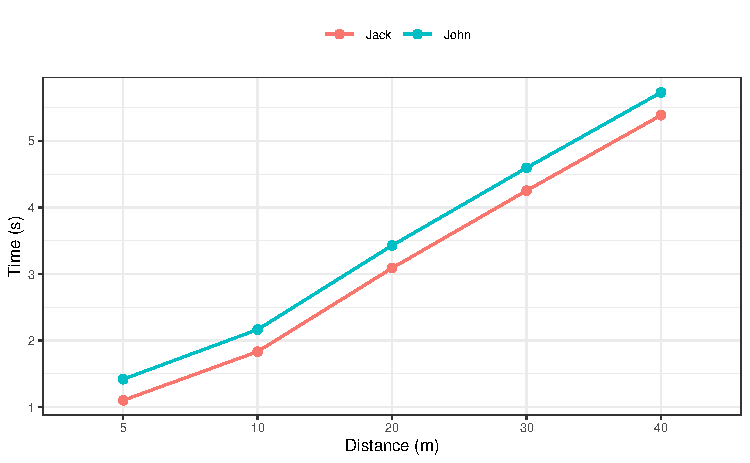
\includegraphics[width=0.9\linewidth]{paper_files/figure-latex/unnamed-chunk-25-1} \end{center}

\normalsize

Using the following code, we can see the differences in estimated MSS and TAU parameters:

\small

\begin{Shaded}
\begin{Highlighting}[]
\CommentTok{\# Since this is a perfect simulation and stats::nls will complain}
\CommentTok{\# we need to add very small noise, or measurement error to the times}
\FunctionTok{set.seed}\NormalTok{(}\DecValTok{1667}\NormalTok{)}
\NormalTok{rand\_noise }\OtherTok{\textless{}{-}} \FunctionTok{rnorm}\NormalTok{(}\FunctionTok{nrow}\NormalTok{(split\_times), }\DecValTok{0}\NormalTok{, }\DecValTok{10}\SpecialCharTok{\^{}{-}}\DecValTok{5}\NormalTok{)}
\NormalTok{split\_times}\SpecialCharTok{$}\NormalTok{john\_time }\OtherTok{\textless{}{-}}\NormalTok{ split\_times}\SpecialCharTok{$}\NormalTok{john\_time }\SpecialCharTok{+}\NormalTok{ rand\_noise}
\NormalTok{split\_times}\SpecialCharTok{$}\NormalTok{jack\_time }\OtherTok{\textless{}{-}}\NormalTok{ split\_times}\SpecialCharTok{$}\NormalTok{jack\_time }\SpecialCharTok{+}\NormalTok{ rand\_noise}

\NormalTok{john\_profile }\OtherTok{\textless{}{-}} \FunctionTok{model\_using\_splits}\NormalTok{(}
  \AttributeTok{distance =}\NormalTok{ split\_times}\SpecialCharTok{$}\NormalTok{distance,}
  \AttributeTok{time =}\NormalTok{ split\_times}\SpecialCharTok{$}\NormalTok{john\_time}
\NormalTok{)}

\NormalTok{jack\_profile }\OtherTok{\textless{}{-}} \FunctionTok{model\_using\_splits}\NormalTok{(}
  \AttributeTok{distance =}\NormalTok{ split\_times}\SpecialCharTok{$}\NormalTok{distance,}
  \AttributeTok{time =}\NormalTok{ split\_times}\SpecialCharTok{$}\NormalTok{jack\_time}
\NormalTok{)}

\NormalTok{sprint\_parameters }\OtherTok{\textless{}{-}} \FunctionTok{rbind}\NormalTok{(}
  \FunctionTok{coef}\NormalTok{(john\_profile),}
  \FunctionTok{coef}\NormalTok{(jack\_profile)}
\NormalTok{)}

\FunctionTok{rownames}\NormalTok{(sprint\_parameters) }\OtherTok{\textless{}{-}} \FunctionTok{c}\NormalTok{(}\StringTok{"John"}\NormalTok{, }\StringTok{"Jack"}\NormalTok{)}

\FunctionTok{kable}\NormalTok{(sprint\_parameters, }\AttributeTok{digits =} \DecValTok{2}\NormalTok{, }\AttributeTok{booktabs =} \ConstantTok{TRUE}\NormalTok{)}
\end{Highlighting}
\end{Shaded}

\begin{tabular}{lrrrrrr}
\toprule
  & MSS & TAU & MAC & PMAX & time\_correction & distance\_correction\\
\midrule
John & 9.00 & 1.3 & 6.92 & 15.6 & 0 & 0\\
Jack & 8.49 & 0.7 & 12.06 & 25.6 & 0 & 0\\
\bottomrule
\end{tabular}

\normalsize

As can be seen from the results, a flying start yields biased estimates, particularly for the TAU, MAC and PMAX.

To explore this further, we have run a simple simulation by increasing Jack's flying start distance from 0 to 1 m and depicting the estimated MSS, TAU, MAC, and PMAX parameters (please refer to the \protect\hyperlink{supplemental-material}{Supplemental material} for the R code).

\small

\begin{center}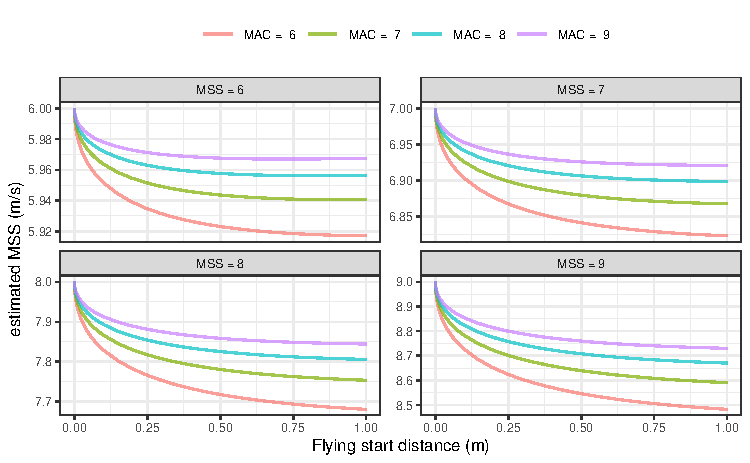
\includegraphics[width=0.9\linewidth]{paper_files/figure-latex/unnamed-chunk-29-1} \end{center}

\normalsize

As can be seen from the figure, MSS is underestimated as flying start distance increases. MAC (and also TAU) are highly affected by the flying start distance, and from the figure we can notice that MAC is overestimated as flying start distance increases. Estimated PMAX is also overestimated as flying start distance increases.

Model residuals are also affected by the flying start distance. The shape of residuals distribution depends on number and splits utilized (e.g., 10, 20, 30, 40 m versus 5, 15, 30 m), but here we can see the effect of the flying start distance on the model residuals per split distance utilized in our simple simulation:

\small

\begin{center}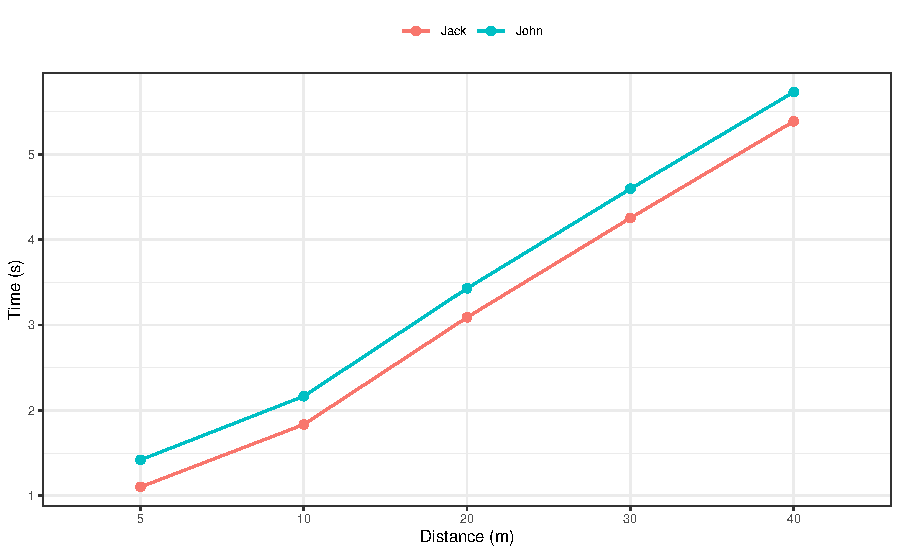
\includegraphics[width=0.9\linewidth]{paper_files/figure-latex/unnamed-chunk-30-1} \end{center}

\normalsize

Another way to visualize the effect of the flying start distance on split distance residuals can be found on the next figure:

\small

\begin{center}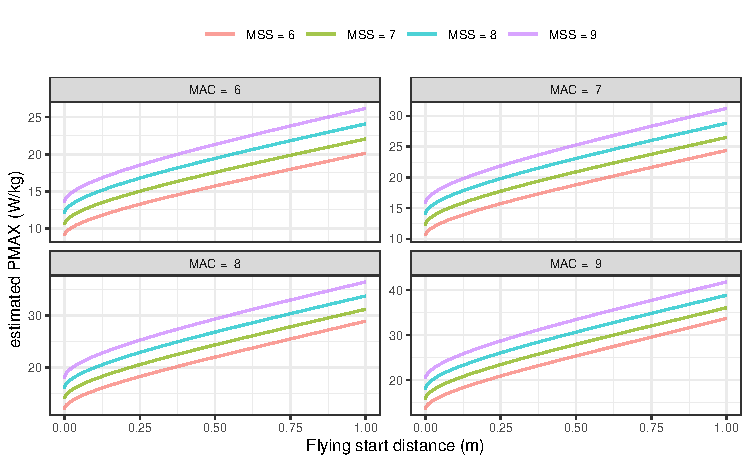
\includegraphics[width=0.9\linewidth]{paper_files/figure-latex/unnamed-chunk-31-1} \end{center}

\normalsize

Clearly, any type of flying start where there is a difference between initial force production and start time can result in biased parameters and predictions. Since maximal sprint speed is difficult to improve, the effects of start inconsistencies can mask effects of the training intervention. It is thus crucial to standardize the start when testing and implementing the following techniques when using the \textbf{shorts} package.

\hypertarget{how-to-overcome-missing-the-initial-force-production-when-using-timing-gates}{%
\subsubsection{How to overcome missing the initial force production when using timing gates?}\label{how-to-overcome-missing-the-initial-force-production-when-using-timing-gates}}

A potential solution is to use a correction factor - the recommendation in the literature is +0.5 s (\protect\hyperlink{ref-haugenSprintMechanicalProperties2020}{Thomas A. Haugen, Breitschädel, and Seiler 2020}, \protect\hyperlink{ref-haugenSprintMechanicalVariables2019}{2019}). Interestingly, the average difference between using timing gates and a block start for 40 m sprint time was 0.27 s (\protect\hyperlink{ref-haugenDifferenceStartImpact2012}{Thomas A. Haugen, Tønnessen, and Seiler 2012}). So, while a timing correction factor is warranted to avoid subsequent errors in estimates of kinetic variables (e.g., overestimate power), a correction factor that is too large will have the opposite effect (e.g., underestimate power).

Rather than providing \emph{apriori} time correction from the literature, \textbf{shorts} package provides an estimation of this parameter from the data provided, together with MSS and TAU. Exactly the same method is suggested by \protect\hyperlink{ref-stenrothForcevelocityProfilingIce2020}{Stenroth, Vartiainen, and Karjalainen} (\protect\hyperlink{ref-stenrothForcevelocityProfilingIce2020}{2020}), named \emph{time shift method}, and the estimated parameter named \emph{time shift parameter}. We have named this parameter \emph{time correction} to be in agreement with the parameter introduced in \protect\hyperlink{problems-with-time-sync-with-radar-gun}{Problems with time sync with radar gun} section of this paper, as well as the available literature.

When implementing time correction, equation \eqref{eq:time-distance} becomes:

\begin{equation}
  t(d) = TAU \times W(-e^{\frac{-d}{MSS \times TAU}} - 1) + \frac{d}{MSS} + TAU - time \; correction \label{eq:time-correction}
\end{equation}

To estimate time correction parameter, we use \texttt{model\_using\_splits\_with\_time\_correction()} function. Here is how we can estimate Jack parameters using either provided time correction (e.g., +0.3 and +0.5 s) or estimated time correction:

\small

\begin{Shaded}
\begin{Highlighting}[]
\NormalTok{jack\_profile\_fixed\_time\_short }\OtherTok{\textless{}{-}} \FunctionTok{model\_using\_splits}\NormalTok{(}
  \AttributeTok{distance =}\NormalTok{ split\_times}\SpecialCharTok{$}\NormalTok{distance,}
  \AttributeTok{time =}\NormalTok{ split\_times}\SpecialCharTok{$}\NormalTok{jack\_time,}
  \AttributeTok{time\_correction =} \FloatTok{0.3}
\NormalTok{)}

\NormalTok{jack\_profile\_fixed\_time\_long }\OtherTok{\textless{}{-}} \FunctionTok{model\_using\_splits}\NormalTok{(}
  \AttributeTok{distance =}\NormalTok{ split\_times}\SpecialCharTok{$}\NormalTok{distance,}
  \AttributeTok{time =}\NormalTok{ split\_times}\SpecialCharTok{$}\NormalTok{jack\_time,}
  \AttributeTok{time\_correction =} \FloatTok{0.5}
\NormalTok{)}

\NormalTok{jack\_profile\_time\_estimated }\OtherTok{\textless{}{-}} \FunctionTok{model\_using\_splits\_with\_time\_correction}\NormalTok{(}
  \AttributeTok{distance =}\NormalTok{ split\_times}\SpecialCharTok{$}\NormalTok{distance,}
  \AttributeTok{time =}\NormalTok{ split\_times}\SpecialCharTok{$}\NormalTok{jack\_time}
\NormalTok{)}

\NormalTok{jack\_parameters }\OtherTok{\textless{}{-}} \FunctionTok{rbind}\NormalTok{(}
  \FunctionTok{coef}\NormalTok{(john\_profile),}
  \FunctionTok{coef}\NormalTok{(jack\_profile),}
  \FunctionTok{coef}\NormalTok{(jack\_profile\_fixed\_time\_short),}
  \FunctionTok{coef}\NormalTok{(jack\_profile\_fixed\_time\_long),}
  \FunctionTok{coef}\NormalTok{(jack\_profile\_time\_estimated)}
\NormalTok{)}

\FunctionTok{rownames}\NormalTok{(jack\_parameters) }\OtherTok{\textless{}{-}} \FunctionTok{c}\NormalTok{(}
  \StringTok{"John"}\NormalTok{,}
  \StringTok{"Jack {-} No corrections"}\NormalTok{,}
  \StringTok{"Jack {-} Fixed time correction (+0.3s)"}\NormalTok{,}
  \StringTok{"Jack {-} Fixed time correction (+0.5s)"}\NormalTok{,}
  \StringTok{"Jack {-} Estimated time correction"}
\NormalTok{)}

\FunctionTok{kable}\NormalTok{(jack\_parameters, }\AttributeTok{digits =} \DecValTok{2}\NormalTok{, }\AttributeTok{booktabs =} \ConstantTok{TRUE}\NormalTok{) }\SpecialCharTok{\%\textgreater{}\%}
  \FunctionTok{kable\_styling}\NormalTok{(}\AttributeTok{latex\_options =} \FunctionTok{c}\NormalTok{(}\StringTok{"scale\_down"}\NormalTok{, }\StringTok{"hold\_position"}\NormalTok{))}
\end{Highlighting}
\end{Shaded}

\begin{table}[!h]
\centering
\resizebox{\linewidth}{!}{
\begin{tabular}{lrrrrrr}
\toprule
  & MSS & TAU & MAC & PMAX & time\_correction & distance\_correction\\
\midrule
John & 9.00 & 1.30 & 6.92 & 15.6 & 0.00 & 0\\
Jack - No corrections & 8.49 & 0.70 & 12.06 & 25.6 & 0.00 & 0\\
Jack - Fixed time correction (+0.3s) & 9.00 & 1.25 & 7.19 & 16.2 & 0.30 & 0\\
Jack - Fixed time correction (+0.5s) & 9.62 & 1.77 & 5.43 & 13.1 & 0.50 & 0\\
Jack - Estimated time correction & 8.96 & 1.22 & 7.37 & 16.5 & 0.28 & 0\\
\bottomrule
\end{tabular}}
\end{table}

\normalsize

In Jack's case, both +0.3 s fixed time correction and time correction estimation yield parameters closer to John's (i.e.~true parameters). We have used these two model definitions in retrospective pilot study (\protect\hyperlink{ref-vescoviSprintMechanicalCharacteristics2021}{Vescovi and Jovanovi'c 2021}), demonstrating statistically significant differences in estimated FVP parameters.

Instead of using time correction as simple intercept in the equation \eqref{eq:time-correction}, we can estimate the \emph{distance correction} (i.e., the flying start distance) using the following equation:

\begin{equation}
  \begin{split}
   t(d) &= (TAU \times W(-e^{\frac{-d + distance \; correction}{MSS \times TAU}} - 1) + \frac{d + distance \; correction}{MSS} + TAU) \\ 
   &\quad-(TAU \times W(-e^{\frac{distance \; correction}{MSS \times TAU}} - 1) + \frac{distance \; correction}{MSS} + TAU) 
   \end{split}
   \label{eq:distance-correction}
\end{equation}

Equation \eqref{eq:distance-correction} was used to generate the data for John and Jack (please refer to the provided R code), as well as for the simple simulation, and can be used as model definition to control for the flying start distance.

To estimate distance correction parameter, we use \texttt{model\_using\_splits\_with\_distance\_correction()} function. Here is how we can estimate Jack parameters using distance correction:

\small

\begin{Shaded}
\begin{Highlighting}[]
\NormalTok{jack\_profile\_distance\_correction }\OtherTok{\textless{}{-}} \FunctionTok{model\_using\_splits\_with\_distance\_correction}\NormalTok{(}
  \AttributeTok{distance =}\NormalTok{ split\_times}\SpecialCharTok{$}\NormalTok{distance,}
  \AttributeTok{time =}\NormalTok{ split\_times}\SpecialCharTok{$}\NormalTok{jack\_time}
\NormalTok{)}

\NormalTok{jack\_parameters }\OtherTok{\textless{}{-}} \FunctionTok{rbind}\NormalTok{(}
\NormalTok{  jack\_parameters,}
  \FunctionTok{coef}\NormalTok{(jack\_profile\_distance\_correction)}
\NormalTok{)}

\FunctionTok{rownames}\NormalTok{(jack\_parameters) [}\DecValTok{6}\NormalTok{] }\OtherTok{\textless{}{-}} \StringTok{"Jack {-} Estimated distance correction"}

\FunctionTok{kable}\NormalTok{(jack\_parameters, }\AttributeTok{digits =} \DecValTok{2}\NormalTok{, }\AttributeTok{booktabs =} \ConstantTok{TRUE}\NormalTok{) }\SpecialCharTok{\%\textgreater{}\%}
  \FunctionTok{kable\_styling}\NormalTok{(}\AttributeTok{latex\_options =} \FunctionTok{c}\NormalTok{(}\StringTok{"scale\_down"}\NormalTok{, }\StringTok{"hold\_position"}\NormalTok{))}
\end{Highlighting}
\end{Shaded}

\begin{table}[!h]
\centering
\resizebox{\linewidth}{!}{
\begin{tabular}{lrrrrrr}
\toprule
  & MSS & TAU & MAC & PMAX & time\_correction & distance\_correction\\
\midrule
John & 9.00 & 1.30 & 6.92 & 15.6 & 0.00 & 0.0\\
Jack - No corrections & 8.49 & 0.70 & 12.06 & 25.6 & 0.00 & 0.0\\
Jack - Fixed time correction (+0.3s) & 9.00 & 1.25 & 7.19 & 16.2 & 0.30 & 0.0\\
Jack - Fixed time correction (+0.5s) & 9.62 & 1.77 & 5.43 & 13.1 & 0.50 & 0.0\\
Jack - Estimated time correction & 8.96 & 1.22 & 7.37 & 16.5 & 0.28 & 0.0\\
\addlinespace
Jack - Estimated distance correction & 9.00 & 1.30 & 6.92 & 15.6 & 0.00 & 0.5\\
\bottomrule
\end{tabular}}
\end{table}

\normalsize

Another model definition, which also represents a novel approach implemented in the \textbf{shorts} package, is to utilize both time and distance corrections. Thus, equation \eqref{eq:time-correction} becomes:

\begin{equation}
  t(d) = TAU \times W(-e^{\frac{-d + distance \; correction}{MSS \times TAU}} - 1) + \frac{d + distance \; correction}{MSS} + TAU - time \; correction \label{eq:time-distance-correction}
\end{equation}

This model is implemented in \texttt{model\_using\_splits\_with\_corrections()} function. Below are the model estimates:

\small

\begin{Shaded}
\begin{Highlighting}[]
\NormalTok{jack\_profile\_time\_distance\_correction }\OtherTok{\textless{}{-}} \FunctionTok{model\_using\_splits\_with\_corrections}\NormalTok{(}
  \AttributeTok{distance =}\NormalTok{ split\_times}\SpecialCharTok{$}\NormalTok{distance,}
  \AttributeTok{time =}\NormalTok{ split\_times}\SpecialCharTok{$}\NormalTok{jack\_time}
\NormalTok{)}

\NormalTok{jack\_parameters }\OtherTok{\textless{}{-}} \FunctionTok{rbind}\NormalTok{(}
\NormalTok{  jack\_parameters,}
  \FunctionTok{coef}\NormalTok{(jack\_profile\_time\_distance\_correction)}
\NormalTok{)}

\FunctionTok{rownames}\NormalTok{(jack\_parameters) [}\DecValTok{7}\NormalTok{] }\OtherTok{\textless{}{-}} 
  \StringTok{"Jack {-} Estimated time \& distance corrections"}

\FunctionTok{kable}\NormalTok{(jack\_parameters, }\AttributeTok{digits =} \DecValTok{2}\NormalTok{, }\AttributeTok{booktabs =} \ConstantTok{TRUE}\NormalTok{) }\SpecialCharTok{\%\textgreater{}\%}
  \FunctionTok{kable\_styling}\NormalTok{(}\AttributeTok{latex\_options =} \FunctionTok{c}\NormalTok{(}\StringTok{"scale\_down"}\NormalTok{, }\StringTok{"hold\_position"}\NormalTok{))}
\end{Highlighting}
\end{Shaded}

\begin{table}[!h]
\centering
\resizebox{\linewidth}{!}{
\begin{tabular}{lrrrrrr}
\toprule
  & MSS & TAU & MAC & PMAX & time\_correction & distance\_correction\\
\midrule
John & 9.00 & 1.30 & 6.92 & 15.6 & 0.00 & 0.0\\
Jack - No corrections & 8.49 & 0.70 & 12.06 & 25.6 & 0.00 & 0.0\\
Jack - Fixed time correction (+0.3s) & 9.00 & 1.25 & 7.19 & 16.2 & 0.30 & 0.0\\
Jack - Fixed time correction (+0.5s) & 9.62 & 1.77 & 5.43 & 13.1 & 0.50 & 0.0\\
Jack - Estimated time correction & 8.96 & 1.22 & 7.37 & 16.5 & 0.28 & 0.0\\
\addlinespace
Jack - Estimated distance correction & 9.00 & 1.30 & 6.92 & 15.6 & 0.00 & 0.5\\
Jack - Estimated time \& distance corrections & 9.00 & 1.30 & 6.92 & 15.6 & 0.40 & 0.5\\
\bottomrule
\end{tabular}}
\end{table}

\normalsize

As can be seen from the results, adding distance correction results in correctly estimating Jack's sprint parameters. There are a few issues with this model definition. Besides being novel and still not validated with actual data, distance correction model has four parameters to estimate, which implies that at least four sprint splits are needed. This imposes practical limitations, since acquiring five timing gates (one for the start and four for splits) might be practically troublesome. One strategy that is sometimes implemented is adding zeros to the sample (i.e., \(t=0\) and \(d=0\)), which increase the number of observations. Unfortunately, this strategy should not be implemented since it will bias the estimated parameters:

\small

\begin{Shaded}
\begin{Highlighting}[]
\NormalTok{jack\_profile\_zero }\OtherTok{\textless{}{-}} \FunctionTok{model\_using\_splits}\NormalTok{(}
  \AttributeTok{distance =} \FunctionTok{c}\NormalTok{(}\DecValTok{0}\NormalTok{, split\_times}\SpecialCharTok{$}\NormalTok{distance),}
  \AttributeTok{time =} \FunctionTok{c}\NormalTok{(}\DecValTok{0}\NormalTok{, split\_times}\SpecialCharTok{$}\NormalTok{jack\_time)}
\NormalTok{)}

\NormalTok{jack\_profile\_time\_estimated\_zero }\OtherTok{\textless{}{-}} \FunctionTok{model\_using\_splits\_with\_time\_correction}\NormalTok{(}
  \AttributeTok{distance =} \FunctionTok{c}\NormalTok{(}\DecValTok{0}\NormalTok{, split\_times}\SpecialCharTok{$}\NormalTok{distance),}
  \AttributeTok{time =} \FunctionTok{c}\NormalTok{(}\DecValTok{0}\NormalTok{, split\_times}\SpecialCharTok{$}\NormalTok{jack\_time)}
\NormalTok{)}

\NormalTok{adding\_zero\_issue }\OtherTok{\textless{}{-}} \FunctionTok{rbind}\NormalTok{(}
  \FunctionTok{coef}\NormalTok{(jack\_profile),}
  \FunctionTok{coef}\NormalTok{(jack\_profile\_zero),}
  \FunctionTok{coef}\NormalTok{(jack\_profile\_time\_estimated),}
  \FunctionTok{coef}\NormalTok{(jack\_profile\_time\_estimated\_zero)}
\NormalTok{)}

\FunctionTok{rownames}\NormalTok{(adding\_zero\_issue) }\OtherTok{\textless{}{-}} \FunctionTok{c}\NormalTok{(}
  \StringTok{"Jack {-} No corrections"}\NormalTok{,}
  \StringTok{"Jack {-} No corrections with zeros added"}\NormalTok{,}
  \StringTok{"Jack {-} Estimated time correction"}\NormalTok{,}
  \StringTok{"Jack profile {-} Estimated time correction with added zeros"}\NormalTok{)}

\FunctionTok{kable}\NormalTok{(adding\_zero\_issue, }\AttributeTok{digits =} \DecValTok{2}\NormalTok{, }\AttributeTok{booktabs =} \ConstantTok{TRUE}\NormalTok{) }\SpecialCharTok{\%\textgreater{}\%}
  \FunctionTok{kable\_styling}\NormalTok{(}\AttributeTok{latex\_options =} \FunctionTok{c}\NormalTok{(}\StringTok{"scale\_down"}\NormalTok{, }\StringTok{"hold\_position"}\NormalTok{))}
\end{Highlighting}
\end{Shaded}

\begin{table}[!h]
\centering
\resizebox{\linewidth}{!}{
\begin{tabular}{lrrrrrr}
\toprule
  & MSS & TAU & MAC & PMAX & time\_correction & distance\_correction\\
\midrule
Jack - No corrections & 8.49 & 0.70 & 12.06 & 25.6 & 0.00 & 0\\
Jack - No corrections with zeros added & 8.49 & 0.70 & 12.06 & 25.6 & 0.00 & 0\\
Jack - Estimated time correction & 8.96 & 1.22 & 7.37 & 16.5 & 0.28 & 0\\
Jack profile - Estimated time correction with added zeros & 8.51 & 0.73 & 11.65 & 24.8 & 0.02 & 0\\
\bottomrule
\end{tabular}}
\end{table}

\normalsize

Adding zeros to the sample nullifies the potential benefits of using time correction model and should be avoided in practice.

It is important to note that using \texttt{predict\_XXX()} family of functions with distance correction model and using estimated distance correction parameter will yield wrong predictions on the original scale (but not on the \emph{theoretical} scale in which force production starts at d=0m and t=0s). This is because \texttt{predict\_XXX()} family of functions utilize equation \eqref{eq:time-distance-correction} and its derivates and integrals, which works for the uncorrected model (time and distance correction parameters are equal to zero), time correction models (distance correction parameter is equal to zero), and time and distance corrections model. You can notice that equations \eqref{eq:time-correction} and \eqref{eq:time-distance-correction} are equivalent to the \eqref{eq:time-distance} equation when time and distance correction parameters are equal to zero. Unfortunately, this doesn't work for the distance correction model when estimated distance correction parameter is used since model definition outlined in the equation \eqref{eq:distance-correction} is different that the equation \eqref{eq:time-distance-correction} when estimated distance correction parameter is different than zero. The solution is to use generic S3 \texttt{predict()} function, but this only predicts split times at split distances.

\small

\begin{Shaded}
\begin{Highlighting}[]
\CommentTok{\# Jack\textquotesingle{}s observed times}
\NormalTok{split\_times}\SpecialCharTok{$}\NormalTok{jack\_time}
\CommentTok{\#\textgreater{} [1] 1.10 1.83 3.09 4.25 5.39}

\CommentTok{\# To predict at "theoretical" distance scale}
\CommentTok{\#  (where force application starts at d=0m)}
\FunctionTok{predict\_time\_at\_distance}\NormalTok{(}
  \AttributeTok{distance =}\NormalTok{ split\_times}\SpecialCharTok{$}\NormalTok{distance, }
  \AttributeTok{MSS =}\NormalTok{ jack\_profile\_time\_estimated}\SpecialCharTok{$}\NormalTok{parameters}\SpecialCharTok{$}\NormalTok{MSS,}
  \AttributeTok{TAU =}\NormalTok{ jack\_profile\_time\_estimated}\SpecialCharTok{$}\NormalTok{parameters}\SpecialCharTok{$}\NormalTok{TAU)}
\CommentTok{\#\textgreater{} [1] 1.38 2.12 3.37 4.54 5.67}

\FunctionTok{predict\_time\_at\_distance}\NormalTok{(}
  \AttributeTok{distance =}\NormalTok{ split\_times}\SpecialCharTok{$}\NormalTok{distance, }
  \AttributeTok{MSS =}\NormalTok{ jack\_profile\_distance\_correction}\SpecialCharTok{$}\NormalTok{parameters}\SpecialCharTok{$}\NormalTok{MSS,}
  \AttributeTok{TAU =}\NormalTok{ jack\_profile\_distance\_correction}\SpecialCharTok{$}\NormalTok{parameters}\SpecialCharTok{$}\NormalTok{TAU)}
\CommentTok{\#\textgreater{} [1] 1.42 2.17 3.43 4.60 5.73}

\CommentTok{\# To predict at original distance scale, use all estimated parameters}
\FunctionTok{predict\_time\_at\_distance}\NormalTok{(}
  \AttributeTok{distance =}\NormalTok{ split\_times}\SpecialCharTok{$}\NormalTok{distance, }
  \AttributeTok{MSS =}\NormalTok{ jack\_profile\_time\_estimated}\SpecialCharTok{$}\NormalTok{parameters}\SpecialCharTok{$}\NormalTok{MSS,}
  \AttributeTok{TAU =}\NormalTok{ jack\_profile\_time\_estimated}\SpecialCharTok{$}\NormalTok{parameters}\SpecialCharTok{$}\NormalTok{TAU,}
  \AttributeTok{time\_correction =}\NormalTok{ jack\_profile\_time\_estimated}\SpecialCharTok{$}\NormalTok{parameters}\SpecialCharTok{$}\NormalTok{time\_correction)}
\CommentTok{\#\textgreater{} [1] 1.10 1.84 3.09 4.25 5.39}

\CommentTok{\# Unfortunately, this doesn\textquotesingle{}t work for the distance correction model}
\FunctionTok{predict\_time\_at\_distance}\NormalTok{(}
  \AttributeTok{distance =}\NormalTok{ split\_times}\SpecialCharTok{$}\NormalTok{distance, }
  \AttributeTok{MSS =}\NormalTok{ jack\_profile\_distance\_correction}\SpecialCharTok{$}\NormalTok{parameters}\SpecialCharTok{$}\NormalTok{MSS,}
  \AttributeTok{TAU =}\NormalTok{ jack\_profile\_distance\_correction}\SpecialCharTok{$}\NormalTok{parameters}\SpecialCharTok{$}\NormalTok{TAU,}
  \AttributeTok{distance\_correction =} 
\NormalTok{    jack\_profile\_distance\_correction}\SpecialCharTok{$}\NormalTok{parameters}\SpecialCharTok{$}\NormalTok{distance\_correction)}
\CommentTok{\#\textgreater{} [1] 1.50 2.23 3.49 4.65 5.78}

\CommentTok{\# Instead use generic S3 predict() function}
\FunctionTok{predict}\NormalTok{(jack\_profile\_distance\_correction)}
\CommentTok{\#\textgreater{} [1] 1.10 1.83 3.09 4.25 5.39}

\FunctionTok{predict}\NormalTok{(}
\NormalTok{  jack\_profile\_distance\_correction}\SpecialCharTok{$}\NormalTok{model,}
  \AttributeTok{newdata =} \FunctionTok{data.frame}\NormalTok{(}\AttributeTok{distance =}\NormalTok{ split\_times}\SpecialCharTok{$}\NormalTok{distance))}
\CommentTok{\#\textgreater{} [1] 1.10 1.83 3.09 4.25 5.39}
\end{Highlighting}
\end{Shaded}

\normalsize

In the next section we examine how these models (no correction, fixed time correction, estimated time correction, estimated distance correction, and estimated time and distance correction) perform using simulated data with varying flying start distance (please refer to the \protect\hyperlink{supplemental-material}{Supplemental material} for the R code).

\small

\normalsize

As can be seen from the next figure, the estimated time correction model estimates MSS almost perfectly, while the estimated distance and estimate time and distance correction models estimates MSS perfectly.

\small

\begin{center}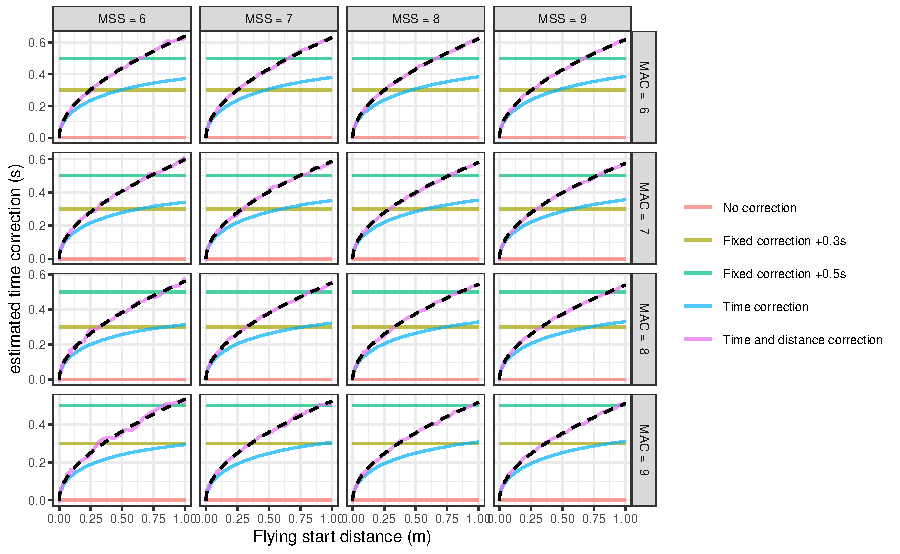
\includegraphics[width=0.9\linewidth]{paper_files/figure-latex/unnamed-chunk-38-1} \end{center}

\normalsize

Similar outcomes are observed for the MAC parameter. The distance correction model and time and distance corrections models performs perfectly, while the time correction model performs almost as good. PMAX demonstrates the same properties as MSS and MAC.

The next figure depicts residuals across split distances for each simulated flying start distance. As can be seen, time correction, distance correction, and time and distance correction models perform much better than the other models.

\small

\begin{Shaded}
\begin{Highlighting}[]
\CommentTok{\# Residuals}
\FunctionTok{ggplot}\NormalTok{(}
\NormalTok{  model\_df,}
  \FunctionTok{aes}\NormalTok{(}
    \AttributeTok{y =}\NormalTok{ residuals,}
    \AttributeTok{x =}\NormalTok{ distance,}
    \AttributeTok{color =}\NormalTok{ flying\_start\_distance,}
    \AttributeTok{group =}\NormalTok{ flying\_start\_distance}
\NormalTok{  )}
\NormalTok{) }\SpecialCharTok{+}
  \FunctionTok{theme\_bw}\NormalTok{(}\DecValTok{8}\NormalTok{) }\SpecialCharTok{+}
  \FunctionTok{geom\_line}\NormalTok{(}\AttributeTok{alpha =} \FloatTok{0.3}\NormalTok{) }\SpecialCharTok{+}
  \FunctionTok{geom\_hline}\NormalTok{(}\AttributeTok{yintercept =} \DecValTok{0}\NormalTok{, }\AttributeTok{linetype =} \StringTok{"dashed"}\NormalTok{) }\SpecialCharTok{+}
  \FunctionTok{scale\_color\_gradientn}\NormalTok{(}\AttributeTok{colours =} \FunctionTok{terrain.colors}\NormalTok{(}\DecValTok{5}\NormalTok{, }\AttributeTok{rev =} \ConstantTok{FALSE}\NormalTok{)) }\SpecialCharTok{+}
  \FunctionTok{facet\_wrap}\NormalTok{(}\SpecialCharTok{\textasciitilde{}}\NormalTok{model) }\SpecialCharTok{+}
  \FunctionTok{xlab}\NormalTok{(}\StringTok{"Distance (m)"}\NormalTok{) }\SpecialCharTok{+}
  \FunctionTok{ylab}\NormalTok{(}\StringTok{"Observed {-} predicted time (s)"}\NormalTok{) }\SpecialCharTok{+}
  \FunctionTok{theme}\NormalTok{(}\AttributeTok{legend.position =} \StringTok{"top"}\NormalTok{) }\SpecialCharTok{+}
  \FunctionTok{labs}\NormalTok{(}\AttributeTok{color =} \StringTok{"Flying start distance"}\NormalTok{)}
\end{Highlighting}
\end{Shaded}

\begin{center}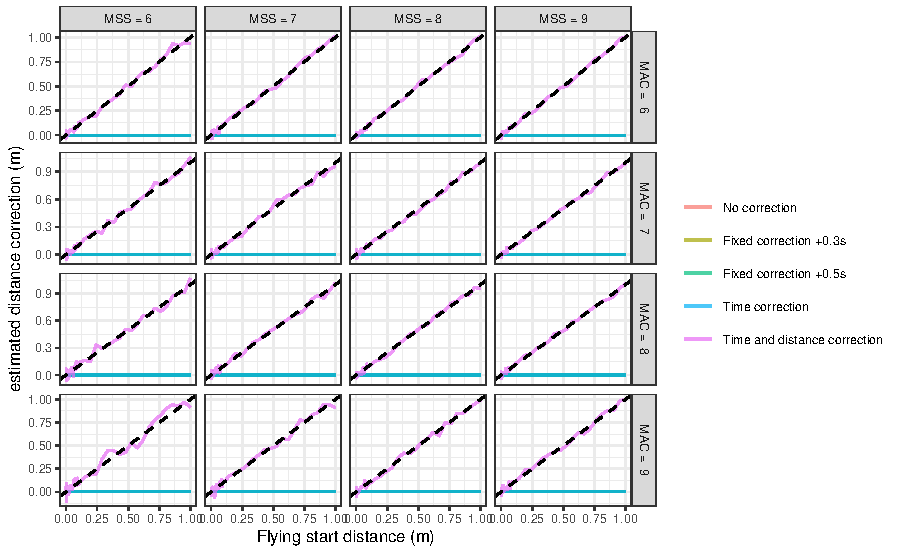
\includegraphics[width=0.9\linewidth]{paper_files/figure-latex/unnamed-chunk-39-1} \end{center}

\normalsize

The outcomes from this simple simulation data clearly demonstrates that the time correction, distance correction, and time and distance correction models represent sound improvements in parameter estimation and model fit compared to no corrections model and fixed correction model when attempting to overcome the flying start issues. Since the time correction and distance correction models are simpler and requires three parameters to be estimated, they might be practically more useful than the time and distance correction model, which requires four parameters estimation and thus more than four timing gates and sprint splits. More elaborate simulation study is currently ongoing and the results will be reported in another paper.

Time correction, distance correction, and time and distance corrections are also implemented in the mixed-models using \texttt{mixed\_model\_using\_splits\_with\_time\_correction()}, \texttt{mixed\_model\_using\_splits\_with\_distance\_correction()}, and \texttt{mixed\_model\_using\_splits\_with\_corrections()} functions. We will showcase their use at the end of this paper.

\hypertarget{leave-one-out-cross-validation}{%
\section{Leave-one-out Cross-Validation}\label{leave-one-out-cross-validation}}

To estimate parameter stability, model over-fitting, and performance on the unseen data, \textbf{shorts} model function comes with implemented \emph{leave-one-out cross validation} (LOOCV) (\protect\hyperlink{ref-jamesIntroductionStatisticalLearning2017}{James et al. 2017}; \protect\hyperlink{ref-jovanovicBmbstatsBootstrapMagnitudebased2020}{Jovanović 2020}; \protect\hyperlink{ref-kuhnAppliedPredictiveModeling2018}{Kuhn and Johnson 2018}). LOOCV involves a simple, yet powerful procedure, of removing each observation, rebuilding the model, and making predictions for that removed observation. This process is repeated for each observation in the model dataset. LOOCV allows one to check estimated parameters stability, and model performance on the unseen data.

Let's perform LOOCV using Jack's data and the time correction model:

\small

\begin{Shaded}
\begin{Highlighting}[]
\NormalTok{jack\_LOOCV }\OtherTok{\textless{}{-}} \FunctionTok{model\_using\_splits\_with\_time\_correction}\NormalTok{(}
  \AttributeTok{distance =}\NormalTok{ split\_times}\SpecialCharTok{$}\NormalTok{distance,}
  \AttributeTok{time =}\NormalTok{ split\_times}\SpecialCharTok{$}\NormalTok{jack\_time,}
  \AttributeTok{LOOCV =} \ConstantTok{TRUE}
\NormalTok{)}
\end{Highlighting}
\end{Shaded}

\normalsize

The model print output provides training dataset estimates and model performance, as well as LOOCV estimates and model performance.

Next we plot estimated parameters across LOOCV folds (please refer to the \protect\hyperlink{supplemental-material}{Supplemental material} for the R code):

\small

\begin{center}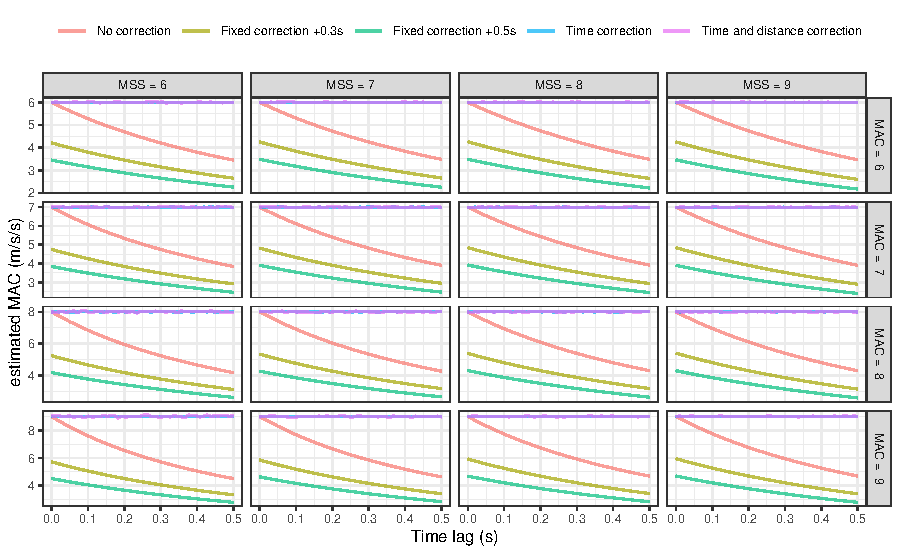
\includegraphics[width=0.9\linewidth]{paper_files/figure-latex/unnamed-chunk-41-1} \end{center}

\normalsize

Here is the plot of the training and LOOCV residuals:

\small

\begin{center}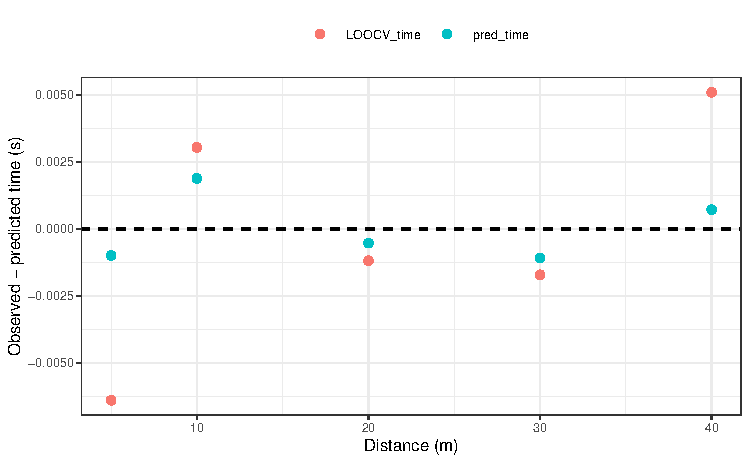
\includegraphics[width=0.9\linewidth]{paper_files/figure-latex/unnamed-chunk-42-1} \end{center}

\normalsize

As expected, the model has more issues predicting unseen split times for both short or long distances. Please note, that since LOOCV removes one observation, if the model estimates three parameters, then at least four observations are needed, since we need to make sure the model can be estimated once a single observation is removed. LOOCV can also be implemented with the mixed-effects models in the \textbf{shorts} package.

\hypertarget{example-analysis}{%
\section{Example analysis}\label{example-analysis}}

Let's utilize demonstrated functionalities of the \textbf{shorts} package using real-world data. The first dataset comes from Usain Bolt's performance from IAAF World Championship held in London, 2017, and the second dataset involve Jason Vescovi's sample data for 52 female soccer and field hockey athletes which comes with the \textbf{shorts} package (see \texttt{?vescovi}).

\hypertarget{usain-bolts-run-from-london-2017}{%
\subsection{Usain Bolt's run from London 2017}\label{usain-bolts-run-from-london-2017}}

The following dataset represents Usain Bolt's race in the finals at the IAAF World Championship held in London, 2017. Since reaction time enters the splits, we want to see how that will affect the model estimates, and particularly, if the estimated time correction model will pick-up reaction time.

For the sake of this analysis, only 10 m splits over 60 m race distance are used.

\small

\begin{Shaded}
\begin{Highlighting}[]
\NormalTok{bolt\_reaction\_time }\OtherTok{\textless{}{-}} \FloatTok{0.183}

\NormalTok{bolt\_distance }\OtherTok{\textless{}{-}} \FunctionTok{c}\NormalTok{(}\DecValTok{10}\NormalTok{, }\DecValTok{20}\NormalTok{, }\DecValTok{30}\NormalTok{, }\DecValTok{40}\NormalTok{, }\DecValTok{50}\NormalTok{, }\DecValTok{60}\NormalTok{)}
\NormalTok{bolt\_time }\OtherTok{\textless{}{-}} \FunctionTok{c}\NormalTok{(}\FloatTok{1.963}\NormalTok{, }\FloatTok{2.983}\NormalTok{, }\FloatTok{3.883}\NormalTok{, }\FloatTok{4.763}\NormalTok{, }\FloatTok{5.643}\NormalTok{, }\FloatTok{6.493}\NormalTok{)}

\CommentTok{\# No corrections model}
\NormalTok{bolt\_m1 }\OtherTok{\textless{}{-}} \FunctionTok{model\_using\_splits}\NormalTok{(}
  \AttributeTok{distance =}\NormalTok{ bolt\_distance,}
  \AttributeTok{time =}\NormalTok{ bolt\_time}
\NormalTok{)}

\CommentTok{\# Model with reaction time as fixed time correction}
\NormalTok{bolt\_m2 }\OtherTok{\textless{}{-}} \FunctionTok{model\_using\_splits}\NormalTok{(}
  \AttributeTok{distance =}\NormalTok{ bolt\_distance,}
  \AttributeTok{time =}\NormalTok{ bolt\_time,}
  \AttributeTok{time\_correction =} \SpecialCharTok{{-}}\NormalTok{bolt\_reaction\_time}
\NormalTok{)}

\CommentTok{\# Model with estimated time correction}
\NormalTok{bolt\_m3 }\OtherTok{\textless{}{-}} \FunctionTok{model\_using\_splits\_with\_time\_correction}\NormalTok{(}
  \AttributeTok{distance =}\NormalTok{ bolt\_distance,}
  \AttributeTok{time =}\NormalTok{ bolt\_time}
\NormalTok{)}

\CommentTok{\# Model with estimated time correction, but deducted reaction time}
\NormalTok{bolt\_m4 }\OtherTok{\textless{}{-}} \FunctionTok{model\_using\_splits\_with\_time\_correction}\NormalTok{(}
  \AttributeTok{distance =}\NormalTok{ bolt\_distance,}
  \AttributeTok{time =}\NormalTok{ bolt\_time }\SpecialCharTok{{-}}\NormalTok{ bolt\_reaction\_time}
\NormalTok{)}

\CommentTok{\# Model with estimated time and distance corrections}
\NormalTok{bolt\_m5 }\OtherTok{\textless{}{-}} \FunctionTok{model\_using\_splits\_with\_corrections}\NormalTok{(}
  \AttributeTok{distance =}\NormalTok{ bolt\_distance,}
  \AttributeTok{time =}\NormalTok{ bolt\_time}
\NormalTok{)}

\CommentTok{\# Model with estimated time and distance corrections and}
\CommentTok{\#  deducted reaction time}
\NormalTok{bolt\_m6 }\OtherTok{\textless{}{-}} \FunctionTok{model\_using\_splits\_with\_corrections}\NormalTok{(}
  \AttributeTok{distance =}\NormalTok{ bolt\_distance,}
  \AttributeTok{time =}\NormalTok{ bolt\_time }\SpecialCharTok{{-}}\NormalTok{ bolt\_reaction\_time}
\NormalTok{)}

\NormalTok{bolt\_model }\OtherTok{\textless{}{-}} \FunctionTok{rbind}\NormalTok{(}
  \FunctionTok{data.frame}\NormalTok{(}
    \AttributeTok{model =} \StringTok{"No correction"}\NormalTok{,}
    \FunctionTok{t}\NormalTok{(}\FunctionTok{coef}\NormalTok{(bolt\_m1))}
\NormalTok{  ),}
  \FunctionTok{data.frame}\NormalTok{(}
    \AttributeTok{model =} \StringTok{"No correction {-} RT"}\NormalTok{,}
    \FunctionTok{t}\NormalTok{(}\FunctionTok{coef}\NormalTok{(bolt\_m2))}
\NormalTok{  ),}
  \FunctionTok{data.frame}\NormalTok{(}
    \AttributeTok{model =} \StringTok{"Time correction"}\NormalTok{,}
    \FunctionTok{t}\NormalTok{(}\FunctionTok{coef}\NormalTok{(bolt\_m3))}
\NormalTok{  ),}
  \FunctionTok{data.frame}\NormalTok{(}
    \AttributeTok{model =} \StringTok{"Time correction {-} RT"}\NormalTok{,}
    \FunctionTok{t}\NormalTok{(}\FunctionTok{coef}\NormalTok{(bolt\_m4))}
\NormalTok{  ),}
  \FunctionTok{data.frame}\NormalTok{(}
    \AttributeTok{model =} \StringTok{"Distance correction"}\NormalTok{,}
    \FunctionTok{t}\NormalTok{(}\FunctionTok{coef}\NormalTok{(bolt\_m5))}
\NormalTok{  ),}
  \FunctionTok{data.frame}\NormalTok{(}
    \AttributeTok{model =} \StringTok{"Distance correction {-} RT"}\NormalTok{,}
    \FunctionTok{t}\NormalTok{(}\FunctionTok{coef}\NormalTok{(bolt\_m6))}
\NormalTok{  )}
\NormalTok{)}

\FunctionTok{kable}\NormalTok{(bolt\_model, }\AttributeTok{digits =} \DecValTok{2}\NormalTok{, }\AttributeTok{booktabs =} \ConstantTok{TRUE}\NormalTok{) }\SpecialCharTok{\%\textgreater{}\%}
  \FunctionTok{kable\_styling}\NormalTok{(}\AttributeTok{latex\_options =} \FunctionTok{c}\NormalTok{(}\StringTok{"scale\_down"}\NormalTok{, }\StringTok{"hold\_position"}\NormalTok{))}
\end{Highlighting}
\end{Shaded}

\begin{table}[!h]
\centering
\resizebox{\linewidth}{!}{
\begin{tabular}{lrrrrrr}
\toprule
model & MSS & TAU & MAC & PMAX & time\_correction & distance\_correction\\
\midrule
No correction & 12.1 & 1.56 & 7.77 & 23.6 & 0.00 & 0.00\\
No correction - RT & 11.7 & 1.21 & 9.74 & 28.6 & -0.18 & 0.00\\
Time correction & 11.7 & 1.20 & 9.76 & 28.6 & -0.18 & 0.00\\
Time correction - RT & 11.7 & 1.20 & 9.76 & 28.6 & 0.00 & 0.00\\
Distance correction & 11.6 & 0.85 & 13.56 & 39.3 & -0.81 & -3.98\\
\addlinespace
Distance correction - RT & 11.6 & 0.85 & 13.56 & 39.3 & -0.63 & -3.98\\
\bottomrule
\end{tabular}}
\end{table}

\normalsize

Here is the model estimate of the time and distance it takes for Bolt to reach 99\% of MSS. Please note that we are not using distance and time correction parameters, since we want these estimates to be on the time/distance scale aligned with the actual sprint start (i.e., theoretical scale), not the measurement scale.

\small

\begin{Shaded}
\begin{Highlighting}[]
\NormalTok{bolt\_model }\OtherTok{\textless{}{-}}\NormalTok{ bolt\_model }\SpecialCharTok{\%\textgreater{}\%}
  \FunctionTok{group\_by}\NormalTok{(model) }\SpecialCharTok{\%\textgreater{}\%}
  \FunctionTok{mutate}\NormalTok{(}
    \AttributeTok{dist\_99\_MSS =} \FunctionTok{find\_velocity\_critical\_distance}\NormalTok{(}
      \AttributeTok{MSS =}\NormalTok{ MSS, }\AttributeTok{TAU =}\NormalTok{ TAU,}
      \CommentTok{\# time\_correction = time\_correction,}
      \CommentTok{\# distance\_correction = distance\_correction,}
      \AttributeTok{percent =} \FloatTok{0.99}
\NormalTok{    ),}
    \AttributeTok{time\_99\_MSS =} \FunctionTok{find\_velocity\_critical\_time}\NormalTok{(}
      \AttributeTok{MSS =}\NormalTok{ MSS, }\AttributeTok{TAU =}\NormalTok{ TAU,}
      \CommentTok{\# time\_correction = time\_correction,}
      \AttributeTok{percent =} \FloatTok{0.99}
\NormalTok{    )}
\NormalTok{  )}

\FunctionTok{kable}\NormalTok{(bolt\_model[}\FunctionTok{c}\NormalTok{(}\DecValTok{1}\NormalTok{, }\DecValTok{8}\NormalTok{, }\DecValTok{9}\NormalTok{)], }\AttributeTok{digits =} \DecValTok{2}\NormalTok{, }\AttributeTok{booktabs =} \ConstantTok{TRUE}\NormalTok{)}
\end{Highlighting}
\end{Shaded}

\begin{tabular}{lrr}
\toprule
model & dist\_99\_MSS & time\_99\_MSS\\
\midrule
No correction & 68.7 & 7.20\\
No correction - RT & 51.1 & 5.55\\
Time correction & 51.0 & 5.54\\
Time correction - RT & 51.0 & 5.54\\
Distance correction & 35.8 & 3.94\\
\addlinespace
Distance correction - RT & 35.8 & 3.94\\
\bottomrule
\end{tabular}

\normalsize

\hypertarget{vescovi-data}{%
\subsection{Vescovi data}\label{vescovi-data}}

The data from Vescovi represents a sub-set of data from a total of 220 high-level female athletes (151 soccer players and 69 field hockey players) (\protect\hyperlink{ref-vescoviSprintMechanicalCharacteristics2021}{Vescovi and Jovanovi'c 2021}). Using a random number generator, a total of 52 players (35 soccer and 17 field hockey) were selected for the sample dataset.

The protocol for assessing linear sprint speed has been described previously (\protect\hyperlink{ref-vescoviImpactMaximumSpeed2014}{Vescovi 2014}, \protect\hyperlink{ref-vescoviLocomotorHeartRateMetabolic2016}{2016}, \protect\hyperlink{ref-vescoviSprintSpeedCharacteristics2012}{2012}) and was identical for each cohort. Briefly, all athletes performed a standardized warm-up that included general exercises such as jogging, shuffling, multi-directional movements, and dynamic stretching exercises. Infrared timing gates (Brower Timing, Utah) were positioned at the start line and at 5, 10, 20, 30, and 35 m at a height of approximately 1.0 m. Participants stood with their lead foot positioned approximately 5 cm behind the initial infrared beam (i.e., start line). Only forward movement was permitted (no leaning or rocking backwards) and timing started when the laser of the starting gate was triggered. The best 35 m time, and all associated split times were kept for analysis.

Below is the mixed-effects models analysis of the dataset.

\small

\begin{Shaded}
\begin{Highlighting}[]
\FunctionTok{data}\NormalTok{(}\StringTok{"vescovi"}\NormalTok{)}

\CommentTok{\# Convert data to long}
\NormalTok{df }\OtherTok{\textless{}{-}}\NormalTok{ vescovi }\SpecialCharTok{\%\textgreater{}\%}
  \FunctionTok{select}\NormalTok{(}\DecValTok{1}\SpecialCharTok{:}\DecValTok{13}\NormalTok{) }\SpecialCharTok{\%\textgreater{}\%}
  \CommentTok{\# slice(1:10) \%\textgreater{}\%}
  \FunctionTok{pivot\_longer}\NormalTok{(}
    \AttributeTok{cols =} \DecValTok{9}\SpecialCharTok{:}\DecValTok{13}\NormalTok{,}
    \AttributeTok{names\_to =} \StringTok{"distance"}\NormalTok{,}
    \AttributeTok{values\_to =} \StringTok{"time"}
\NormalTok{  ) }\SpecialCharTok{\%\textgreater{}\%}
  \FunctionTok{mutate}\NormalTok{(}
    \AttributeTok{distance =} \FunctionTok{as.numeric}\NormalTok{(}\FunctionTok{str\_extract}\NormalTok{(distance, }\StringTok{"\^{}[0{-}9]+"}\NormalTok{))}
\NormalTok{  )}
\end{Highlighting}
\end{Shaded}

\normalsize

The following models were used: (1) no corrections model, (2) fixed time correction model (using 0.3s heuristic rule of thumb), (3) time correction model with time correction as fixed effect, (4) time correction model with time correction as random effect, (5) distance correction model with distance correction as fixed effect, (6) distance correction model with distance correction as random effect, (7) time and distance correction model, (8) time and distance correction model with distance correction as fixed effect (and time correction as random effect), and (9) time and distance correction model with distance and time correction as random effects (please refer to the \protect\hyperlink{supplemental-material}{Supplemental material} for the R code).

\small

\normalsize

The following image represents model fit estimator RSE for each model. As can be seen, RSE is reduced the more flexible the model.

\small

\begin{center}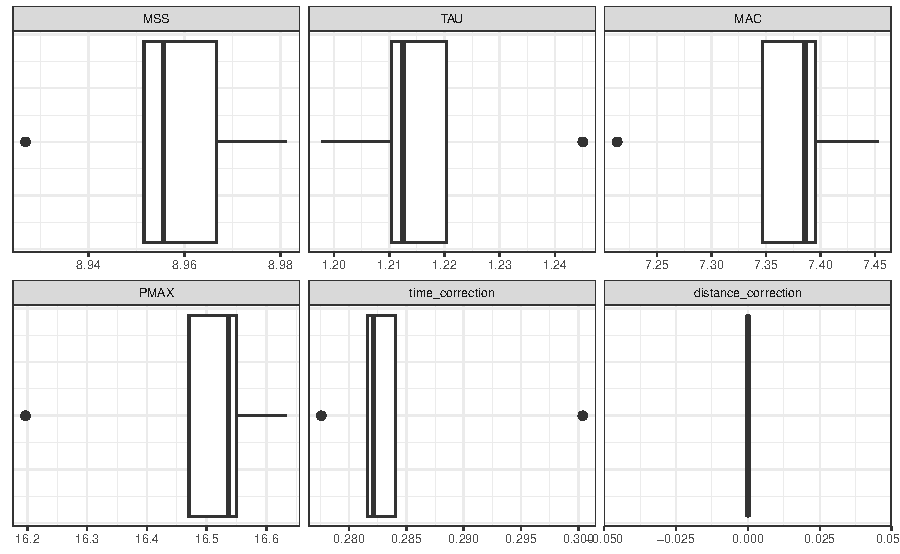
\includegraphics[width=0.9\linewidth]{paper_files/figure-latex/unnamed-chunk-47-1} \end{center}

\normalsize

The following image depicts estimated parameters for each model:

\small

\begin{center}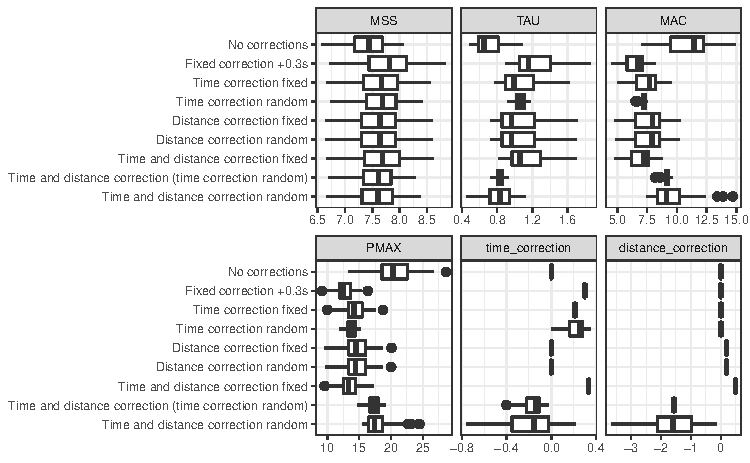
\includegraphics[width=0.9\linewidth]{paper_files/figure-latex/unnamed-chunk-48-1} \end{center}

\normalsize

The following image depicts model residuals across distance splits. To provide practical magnitude of the residuals, we have used between subject observed time SD multiplied with 0.2 and -0.2. This provides practical anchor for the residual magnitude, often referred to as \emph{smallest worthwhile change} (SWC) or \emph{smallest effect size of interest} (SESOI) (\protect\hyperlink{ref-jovanovicBmbstatsBootstrapMagnitudebased2020}{Jovanović 2020}). If the residuals are within this magnitude band, then the model is good in making practically useful predictions. Error bars represent residual bias \(\pm\) 1 SD.

\small

\begin{center}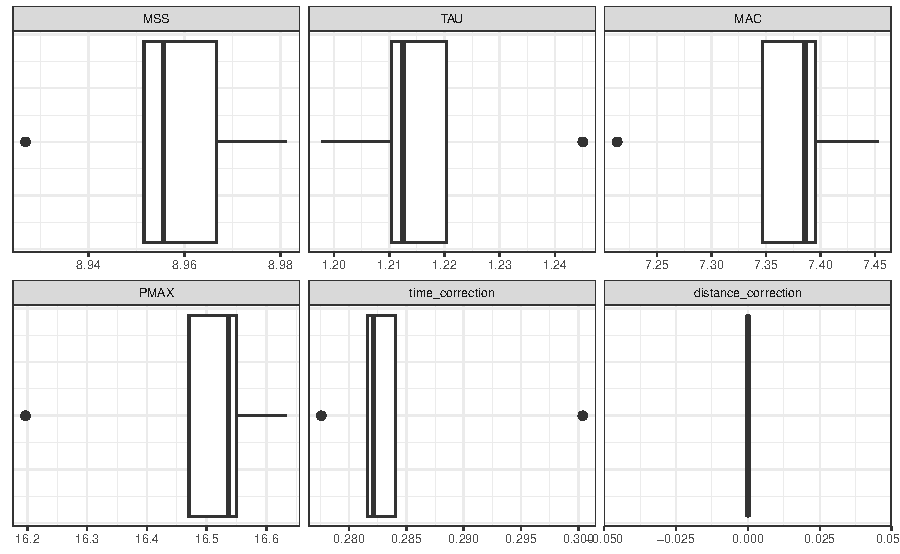
\includegraphics[width=0.9\linewidth]{paper_files/figure-latex/unnamed-chunk-49-1} \end{center}

\normalsize

The following figure depicts model residuals estimators (bias, or mean residual; variance, or SD of the residuals, and MAD, or mean absolute difference).

\small

\begin{center}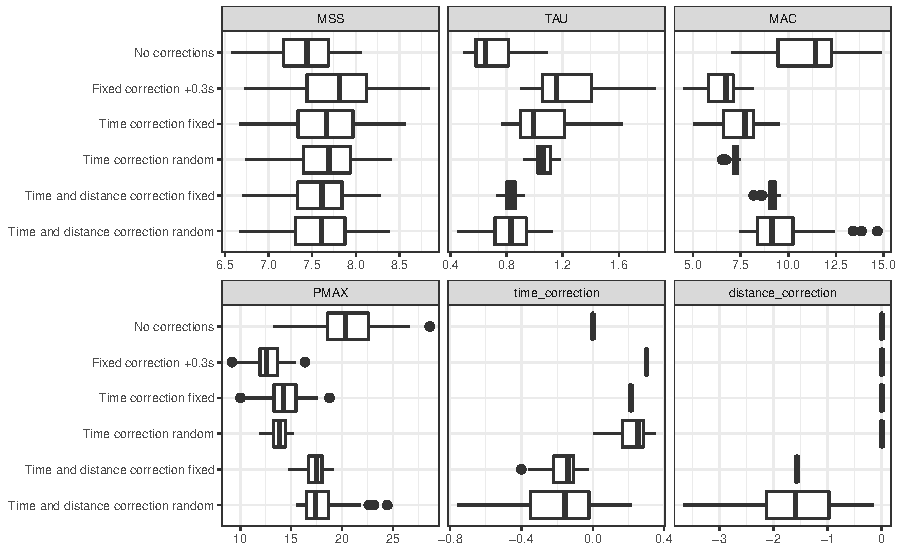
\includegraphics[width=0.9\linewidth]{paper_files/figure-latex/unnamed-chunk-50-1} \end{center}

\normalsize

Which model should be used? Although providing a better fit (using RSE as an estimator of model fit), the time and distance correction models often estimate these parameters that are harder to interpret (e.g., negative distance correction). Although providing novel theoretical models in this paper, we acknowledge the need for validating them in practice, against gold-standard methods, assessing their agreement, as well as their power in detecting and adjusting for timing inconsistencies. More thorough theoretical simulation study is currently in development with the aim to explore the behavior of these models under different scenarios.

We are hoping that the \textbf{shorts} package will help fellow sports scientists and coaches in exploring short sprint profiles and help in driving research, particularly in devising measuring protocols that are sensitive enough to capture training intervention changes, but also robust enough to take into account potential sprint initiation and timing inconsistencies.

\hypertarget{supplemental-material}{%
\section{Supplemental material}\label{supplemental-material}}

The \emph{R Markdown} (\protect\hyperlink{ref-R-bookdown}{Xie 2021a}; \protect\hyperlink{ref-R-rmarkdown}{Allaire et al. 2021}; \protect\hyperlink{ref-rmarkdown2018}{Xie, Allaire, and Grolemund 2018}; \protect\hyperlink{ref-rmarkdown2020}{Xie, Dervieux, and Riederer 2020}) source code for the paper can be found on the GitHub repository: \url{https://github.com/mladenjovanovic/shorts-paper}.

\hypertarget{references}{%
\section*{References}\label{references}}
\addcontentsline{toc}{section}{References}

\hypertarget{refs}{}
\begin{CSLReferences}{1}{0}
\leavevmode\hypertarget{ref-R-rmarkdown}{}%
Allaire, JJ, Yihui Xie, Jonathan McPherson, Javier Luraschi, Kevin Ushey, Aron Atkins, Hadley Wickham, Joe Cheng, Winston Chang, and Richard Iannone. 2021. \emph{Rmarkdown: Dynamic Documents for r}. \url{https://CRAN.R-project.org/package=rmarkdown}.

\leavevmode\hypertarget{ref-altmannDifferentStartingDistances2015}{}%
Altmann, Stefan, Marian Hoffmann, Gunther Kurz, Rainer Neumann, Alexander Woll, and Sascha Haertel. 2015. {``Different {Starting Distances Affect} 5-m {Sprint Times}.''} \emph{Journal of Strength and Conditioning Research} 29 (8): 2361--66. \url{https://doi.org/10.1519/JSC.0000000000000865}.

\leavevmode\hypertarget{ref-altmannValiditySingleBeamTiming2017}{}%
Altmann, Stefan, Max Spielmann, Florian Azad Engel, Rainer Neumann, Steffen Ringhof, Doris Oriwol, and Sascha Haertel. 2017. {``Validity of {Single}-{Beam Timing Lights} at {Different Heights}.''} \emph{Journal of Strength and Conditioning Research} 31 (7): 1994--99. \url{https://doi.org/10.1519/JSC.0000000000001889}.

\leavevmode\hypertarget{ref-altmannAccuracySingleBeam2018}{}%
Altmann, Stefan, Max Spielmann, Florian Azad Engel, Steffen Ringhof, Doris Oriwol, Sascha Härtel, and Rainer Neumann. 2018. {``Accuracy of Single Beam Timing Lights for Determining Velocities in a Flying 20-m Sprint: {Does} Timing Light Height Matter?''} \emph{Journal of Human Sport and Exercise} 13 (3). \url{https://doi.org/10.14198/jhse.2018.133.10}.

\leavevmode\hypertarget{ref-arsacModelingEnergetics100m2002}{}%
Arsac, Laurent M., and Elio Locatelli. 2002. {``Modeling the Energetics of 100-m Running by Using Speed Curves of World Champions.''} \emph{Journal of Applied Physiology} 92 (5): 1781--88. \url{https://doi.org/10.1152/japplphysiol.00754.2001}.

\leavevmode\hypertarget{ref-batesNonlinearModels1992}{}%
Bates, D. M., and J. M. Chambers. 1992. {``Nonlinear Models.''} In \emph{Statistical {Models} in {S}}. {Wadsworth \& Brooks/Cole}.

\leavevmode\hypertarget{ref-batesNonlinearRegressionAnalysis2007}{}%
Bates, Douglas M., and Donald G. Watts. 2007. \emph{Nonlinear Regression Analysis and Its Applications}. Wiley Series in Probability and Mathematical Statistics. {New York, NY}: {Wiley}.

\leavevmode\hypertarget{ref-brownAssessmentLinearSprinting2004}{}%
Brown, Todd D., Jason D. Vescovi, and Jaci L. Vanheest. 2004. {``Assessment of Linear Sprinting Performance: A Theoretical Paradigm.''} \emph{Journal of Sports Science \& Medicine} 3 (4): 203--10.

\leavevmode\hypertarget{ref-buchheitMechanicalDeterminantsAcceleration2014}{}%
Buchheit, Martin, Pierre Samozino, Jonathan Alexander Glynn, Ben Simpson Michael, Hani Al Haddad, Alberto Mendez-Villanueva, and Jean Benoit Morin. 2014. {``Mechanical Determinants of Acceleration and Maximal Sprinting Speed in Highly Trained Young Soccer Players.''} \emph{Journal of Sports Sciences} 32 (20): 1906--13. \url{https://doi.org/10.1080/02640414.2014.965191}.

\leavevmode\hypertarget{ref-clarkNFLCombine40Yard2017}{}%
Clark, Kenneth P., Randall H. Rieger, Richard F. Bruno, and David J. Stearne. 2017. {``The {NFL Combine} 40-{Yard Dash}: {How Important} Is {Maximum Velocity}?''} \emph{Journal of Strength and Conditioning Research}, June, 1. \url{https://doi.org/10.1519/JSC.0000000000002081}.

\leavevmode\hypertarget{ref-edwardsSprintAccelerationCharacteristics2020}{}%
Edwards, Toby, Benjamin Piggott, Harry G. Banyard, G. Gregory Haff, and Christopher Joyce. 2020. {``Sprint Acceleration Characteristics Across the {Australian} Football Participation Pathway.''} \emph{Sports Biomechanics}, August, 1--13. \url{https://doi.org/10.1080/14763141.2020.1790641}.

\leavevmode\hypertarget{ref-doi:10.1098ux2frspb.1927.0035}{}%
Furusawa, K., Archibald Vivian Hill, and J. L. Parkinson. 1927. {``The Dynamics of "Sprint" Running.''} \emph{Proceedings of the Royal Society of London. Series B, Containing Papers of a Biological Character} 102 (713): 29--42. \url{https://doi.org/10.1098/rspb.1927.0035}.

\leavevmode\hypertarget{ref-R-LambertW}{}%
Goerg, Georg M. 2020. \emph{LambertW: Probabilistic Models to Analyze and Gaussianize Heavy-Tailed, Skewed Data}. \url{https://CRAN.R-project.org/package=LambertW}.

\leavevmode\hypertarget{ref-haugenPowerForceVelocityProfilingSprinting2020}{}%
Haugen, Thomas A., Felix Breitschädel, and Pierre Samozino. 2020. {``Power-{Force}-{Velocity Profiling} of {Sprinting Athletes}: {Methodological} and {Practical Considerations When Using Timing Gates}.''} \emph{Journal of Strength and Conditioning Research} 34 (6): 1769--73. \url{https://doi.org/10.1519/JSC.0000000000002890}.

\leavevmode\hypertarget{ref-haugenSprintMechanicalVariables2019}{}%
Haugen, Thomas A., Felix Breitschädel, and Stephen Seiler. 2019. {``Sprint Mechanical Variables in Elite Athletes: {Are} Force-Velocity Profiles Sport Specific or Individual?''} Edited by Leonardo A. Peyré-Tartaruga. \emph{PLOS ONE} 14 (7): e0215551. \url{https://doi.org/10.1371/journal.pone.0215551}.

\leavevmode\hypertarget{ref-haugenSprintMechanicalProperties2020}{}%
---------. 2020. {``Sprint Mechanical Properties in Soccer Players According to Playing Standard, Position, Age and Sex.''} \emph{Journal of Sports Sciences} 38 (9): 1070--76. \url{https://doi.org/10.1080/02640414.2020.1741955}.

\leavevmode\hypertarget{ref-haugenDifferenceStartImpact2012}{}%
Haugen, Thomas A, Espen Tønnessen, and Stephen K Seiler. 2012. {``The {Difference Is} in the {Start}: {Impact} of {Timing} and {Start Procedure} on {Sprint Running Performance}:''} \emph{Journal of Strength and Conditioning Research} 26 (2): 473--79. \url{https://doi.org/10.1519/JSC.0b013e318226030b}.

\leavevmode\hypertarget{ref-haugenSprintRunningPerformance2016}{}%
Haugen, Thomas, and Martin Buchheit. 2016. {``Sprint {Running Performance Monitoring}: {Methodological} and {Practical Considerations}.''} \emph{Sports Medicine} 46 (5): 641--56. \url{https://doi.org/10.1007/s40279-015-0446-0}.

\leavevmode\hypertarget{ref-jamesIntroductionStatisticalLearning2017}{}%
James, Gareth, Daniela Witten, Trevor Hastie, and Robert Tibshirani. 2017. \emph{An {Introduction} to {Statistical Learning}: With {Applications} in {R}}. 1st ed. 2013, Corr. 7th printing 2017 edition. {New York}: {Springer}.

\leavevmode\hypertarget{ref-jimenez-reyesRelationshipVerticalHorizontal2018}{}%
Jiménez-Reyes, Pedro, Pierre Samozino, Amador García-Ramos, Víctor Cuadrado-Peñafiel, Matt Brughelli, and Jean-Benoît Morin. 2018. {``Relationship Between Vertical and Horizontal Force-Velocity-Power Profiles in Various Sports and Levels of Practice.''} \emph{PeerJ} 6 (November): e5937. \url{https://doi.org/10.7717/peerj.5937}.

\leavevmode\hypertarget{ref-jovanovicBmbstatsBootstrapMagnitudebased2020}{}%
Jovanović, Mladen. 2020. \emph{Bmbstats: {Bootstrap Magnitude}-Based {Statistics} for {Sports Scientists}}. {Mladen Jovanović}.

\leavevmode\hypertarget{ref-R-shorts}{}%
---------. 2021. \emph{Shorts: Short Sprints}. \url{https://mladenjovanovic.github.io/shorts/}.

\leavevmode\hypertarget{ref-kuhnAppliedPredictiveModeling2018}{}%
Kuhn, Max, and Kjell Johnson. 2018. \emph{Applied {Predictive Modeling}}. 1st ed. 2013, Corr. 2nd printing 2016 edition. {New York}: {Springer}.

\leavevmode\hypertarget{ref-mangineSpeedForcePower2014}{}%
Mangine, Gerald T., Jay R. Hoffman, Adam M. Gonzalez, Adam J. Wells, Jeremy R. Townsend, Adam R. Jajtner, William P. McCormack, et al. 2014. {``Speed, {Force}, and {Power Values Produced From Nonmotorized Treadmill Test Are Related} to {Sprinting Performance}:''} \emph{Journal of Strength and Conditioning Research} 28 (7): 1812--19. \url{https://doi.org/10.1519/JSC.0000000000000316}.

\leavevmode\hypertarget{ref-marcote-pequenoAssociationForceVelocity2019}{}%
Marcote-Pequeño, Ramón, Amador García-Ramos, Víctor Cuadrado-Peñafiel, Jorge M. González-Hernández, Miguel Ángel Gómez, and Pedro Jiménez-Reyes. 2019. {``Association {Between} the {Force}{{Velocity Profile}} and {Performance Variables Obtained} in {Jumping} and {Sprinting} in {Elite Female Soccer Players}.''} \emph{International Journal of Sports Physiology and Performance} 14 (2): 209--15. \url{https://doi.org/10.1123/ijspp.2018-0233}.

\leavevmode\hypertarget{ref-morinSpreadsheetSprintAcceleration2017}{}%
Morin, J. B. 2017. {``A Spreadsheet for {Sprint} Acceleration {Force}-{Velocity}-{Power} Profiling.''} {JB Morin, PhD - Sport Science}. December 13, 2017. \url{https://jbmorin.net/2017/12/13/a-spreadsheet-for-sprint-acceleration-force-velocity-power-profiling/}.

\leavevmode\hypertarget{ref-morinInterpretingPowerForceVelocityProfiles2016}{}%
Morin, Jean-Benoit, and Pierre Samozino. 2016. {``Interpreting {Power}-{Force}-{Velocity Profiles} for {Individualized} and {Specific Training}.''} \emph{International Journal of Sports Physiology and Performance} 11 (2): 267--72. \url{https://doi.org/10.1123/ijspp.2015-0638}.

\leavevmode\hypertarget{ref-morinSpreadsheetSprintAcceleration2019}{}%
---------. 2019. {``Spreadsheet for {Sprint} Acceleration Force-Velocity-Power Profiling.''}

\leavevmode\hypertarget{ref-morinSimpleMethodComputing2019}{}%
Morin, Jean-Benoit, Pierre Samozino, Munenori Murata, Matt R Cross, and Ryu Nagahara. 2019. {``A Simple Method for Computing Sprint Acceleration Kinetics from Running Velocity Data: {Replication} Study with Improved Design.''} \emph{Journal of Biomechanics} 94 (September): 82--87. \url{https://doi.org/10.1016/j.jbiomech.2019.07.020}.

\leavevmode\hypertarget{ref-motulskyIntuitiveBiostatisticsNonmathematical2018}{}%
Motulsky, Harvey. 2018. \emph{Intuitive Biostatistics: A Nonmathematical Guide to Statistical Thinking}. Fourth edition. {New York}: {Oxford University Press}.

\leavevmode\hypertarget{ref-R-nlme}{}%
Pinheiro, José, Douglas Bates, and R-core. 2021. \emph{Nlme: Linear and Nonlinear Mixed Effects Models}. \url{https://svn.r-project.org/R-packages/trunk/nlme/}.

\leavevmode\hypertarget{ref-R-base}{}%
R Core Team. 2020. \emph{R: A Language and Environment for Statistical Computing}. Vienna, Austria: R Foundation for Statistical Computing. \url{https://www.R-project.org/}.

\leavevmode\hypertarget{ref-samozinoSimpleMethodMeasuring2016}{}%
Samozino, P., G. Rabita, S. Dorel, J. Slawinski, N. Peyrot, E. Saez de Villarreal, and J.-B. Morin. 2016. {``A Simple Method for Measuring Power, Force, Velocity Properties, and Mechanical Effectiveness in Sprint Running: {Simple} Method to Compute Sprint Mechanics.''} \emph{Scandinavian Journal of Medicine \& Science in Sports} 26 (6): 648--58. \url{https://doi.org/10.1111/sms.12490}.

\leavevmode\hypertarget{ref-stenrothSpreadsheetSprintAcceleration2020}{}%
Stenroth, Lauri, and Paavo Vartiainen. 2020. {``Spreadsheet for Sprint Acceleration Force-Velocity-Power Profiling with Optimization to Correct Start Time.''} \url{https://doi.org/10.13140/RG.2.2.12841.83045}.

\leavevmode\hypertarget{ref-stenrothForcevelocityProfilingIce2020}{}%
Stenroth, Lauri, Paavo Vartiainen, and Pasi A. Karjalainen. 2020. {``Force-Velocity Profiling in Ice Hockey Skating: Reliability and Validity of a Simple, Low-Cost Field Method.''} \emph{Sports Biomechanics}, June, 1--16. \url{https://doi.org/10.1080/14763141.2020.1770321}.

\leavevmode\hypertarget{ref-vaningenschenauCanCyclePower1991}{}%
van Ingen Schenau, Gerrit Jan, Ron Jacobs, and Jos J. de Koning. 1991. {``Can Cycle Power Predict Sprint Running Performance?''} \emph{European Journal of Applied Physiology and Occupational Physiology} 63 (3-4): 255--60. \url{https://doi.org/10.1007/BF00233857}.

\leavevmode\hypertarget{ref-vescoviSprintSpeedCharacteristics2012}{}%
Vescovi, Jason D. 2012. {``Sprint Speed Characteristics of High-Level {American} Female Soccer Players: {Female Athletes} in {Motion} ({FAiM}) {Study}.''} \emph{Journal of Science and Medicine in Sport} 15 (5): 474--78. \url{https://doi.org/10.1016/j.jsams.2012.03.006}.

\leavevmode\hypertarget{ref-vescoviImpactMaximumSpeed2014}{}%
---------. 2014. {``Impact of {Maximum Speed} on {Sprint Performance During High}-{Level Youth Female Field Hockey Matches}: {Female Athletes} in {Motion} ({FAiM}) {Study}.''} \emph{International Journal of Sports Physiology and Performance} 9 (4): 621--26. \url{https://doi.org/10.1123/ijspp.2013-0263}.

\leavevmode\hypertarget{ref-vescoviLocomotorHeartRateMetabolic2016}{}%
---------. 2016. {``Locomotor, {Heart}-{Rate}, and {Metabolic Power Characteristics} of {Youth Women}'s {Field Hockey}: {Female Athletes} in {Motion} ({FAiM}) {Study}.''} \emph{Research Quarterly for Exercise and Sport} 87 (1): 68--77. \url{https://doi.org/10.1080/02701367.2015.1124972}.

\leavevmode\hypertarget{ref-vescoviSprintMechanicalCharacteristics2021}{}%
Vescovi, Jason D., and Mladen Jovanovi'c. 2021. {``Sprint {Mechanical Characteristics} of {Female Soccer Players}: {A Retrospective Pilot Study} to {Examine} a {Novel Approach} for {Correction} of {Timing Gate Starts}.''} \emph{Frontiers in Sports and Active Living} 3 (May): 629694. \url{https://doi.org/10.3389/fspor.2021.629694}.

\leavevmode\hypertarget{ref-ward-smithEnergyConversionStrategies2001}{}%
Ward-Smith, A. J. 2001. {``Energy Conversion Strategies During 100 m Sprinting.''} \emph{Journal of Sports Sciences} 19 (9): 701--10. \url{https://doi.org/10.1080/02640410152475838}.

\leavevmode\hypertarget{ref-R-tidyr}{}%
Wickham, Hadley. 2021a. \emph{Tidyr: Tidy Messy Data}. \url{https://CRAN.R-project.org/package=tidyr}.

\leavevmode\hypertarget{ref-R-tidyverse}{}%
---------. 2021b. \emph{Tidyverse: Easily Install and Load the Tidyverse}. \url{https://CRAN.R-project.org/package=tidyverse}.

\leavevmode\hypertarget{ref-R-ggplot2}{}%
Wickham, Hadley, Winston Chang, Lionel Henry, Thomas Lin Pedersen, Kohske Takahashi, Claus Wilke, Kara Woo, Hiroaki Yutani, and Dewey Dunnington. 2021. \emph{Ggplot2: Create Elegant Data Visualisations Using the Grammar of Graphics}. \url{https://CRAN.R-project.org/package=ggplot2}.

\leavevmode\hypertarget{ref-R-dplyr}{}%
Wickham, Hadley, Romain François, Lionel Henry, and Kirill Müller. 2021. \emph{Dplyr: A Grammar of Data Manipulation}. \url{https://CRAN.R-project.org/package=dplyr}.

\leavevmode\hypertarget{ref-knitr2014}{}%
Xie, Yihui. 2014. {``Knitr: A Comprehensive Tool for Reproducible Research in {R}.''} In \emph{Implementing Reproducible Computational Research}, edited by Victoria Stodden, Friedrich Leisch, and Roger D. Peng. Chapman; Hall/CRC. \url{http://www.crcpress.com/product/isbn/9781466561595}.

\leavevmode\hypertarget{ref-knitr2015}{}%
---------. 2015. \emph{Dynamic Documents with {R} and Knitr}. 2nd ed. Boca Raton, Florida: Chapman; Hall/CRC. \url{https://yihui.org/knitr/}.

\leavevmode\hypertarget{ref-R-bookdown}{}%
---------. 2021a. \emph{Bookdown: Authoring Books and Technical Documents with r Markdown}. \url{https://CRAN.R-project.org/package=bookdown}.

\leavevmode\hypertarget{ref-R-knitr}{}%
---------. 2021b. \emph{Knitr: A General-Purpose Package for Dynamic Report Generation in r}. \url{https://yihui.org/knitr/}.

\leavevmode\hypertarget{ref-rmarkdown2018}{}%
Xie, Yihui, J. J. Allaire, and Garrett Grolemund. 2018. \emph{R Markdown: The Definitive Guide}. Boca Raton, Florida: Chapman; Hall/CRC. \url{https://bookdown.org/yihui/rmarkdown}.

\leavevmode\hypertarget{ref-rmarkdown2020}{}%
Xie, Yihui, Christophe Dervieux, and Emily Riederer. 2020. \emph{R Markdown Cookbook}. Boca Raton, Florida: Chapman; Hall/CRC. \url{https://bookdown.org/yihui/rmarkdown-cookbook}.

\leavevmode\hypertarget{ref-R-kableExtra}{}%
Zhu, Hao. 2021. \emph{kableExtra: Construct Complex Table with Kable and Pipe Syntax}.

\end{CSLReferences}



\end{document}
